%Preamble
% \documentclass[handout]{beamer}
\documentclass{beamer}

% \usepackage{default}
% \usetheme{default}
% \usecolortheme{dove}

% section in the header
% \useoutertheme{miniframes}
% \useoutertheme{sidebar}

\usepackage{latexsym,xcolor,multicol,booktabs,calligra}


%Defining viterbi template colors
\definecolor{viterbiyellow}{HTML}{E9A000}
\definecolor{viterbired}{HTML}{990000}

%Redefine more fields as required
\newcommand{\viterbititle}[1]{\title{\textcolor{viterbiyellow}{#1}}}
\newcommand{\viterbiauthor}[1]{\author{\textcolor{viterbiyellow}{#1}}}
\newcommand{\viterbidate}[1]{\date{\textcolor{viterbiyellow}{#1}}}

%Change this environment to include any additional formatting required
\newenvironment{viterbiframe}[1]{
\begin{frame}{\textcolor{viterbired}{#1}}
}
{\end{frame}}

%To show the outline slide before each section
\AtBeginSection[]
{
  \begin{viterbiframe}{Outline}
    \tableofcontents[currentsection,currentsubsection]
  \end{viterbiframe}
}


\setbeamertemplate{headline}
{%
\begin{beamercolorbox}{section in head/foot}
\vskip2pt\insertnavigation{\paperwidth}\vskip2pt
\end{beamercolorbox}%
}

\setbeamertemplate{footline}
{
  \leavevmode%
  \hbox{%
%   \begin{beamercolorbox}[wd=.4\paperwidth,ht=2.25ex,dp=1ex,center]{author in head/foot}%
%     \usebeamerfont{author in head/foot}\insertshortauthor
%   \end{beamercolorbox}%
  \begin{beamercolorbox}[wd=.6\paperwidth,ht=2.25ex,dp=1ex,center]{title in head/foot}%
    \usebeamerfont{title in head/foot}\insertshorttitle\hspace*{3em}
    \insertframenumber{} / \inserttotalframenumber\hspace*{1ex}
  \end{beamercolorbox}}%
  \vskip0pt%
}


% Package to manage the bibliography
% \usepackage[backend=biber, style=numeric, sorting=none]{biblatex}
\usepackage[style=verbose,backend=biber]{biblatex}
% \addbibresource{refsSagawa20.bib}
% \bibliographystyle{plain}
\bibliography{refsSagawa20,refs}


\setbeamerfont{footnote}{size=\tiny}


% \usepackage{enumitem}

\usepackage{cleveref}
\usepackage{hyperref}

% %end preamble


% \usepackage{floatrow}
\usepackage{hyperref}
% \usepackage{url}
\usepackage{booktabs}       % professional-quality tables
\usepackage{amsfonts}       % blackboard math symbols
\usepackage{nicefrac}       % compact symbols for 1/2, etc.
\usepackage{xcolor}
\usepackage{amsmath}
\usepackage{amssymb}
\usepackage{amsthm}
\usepackage{caption}
\usepackage{subcaption}
\usepackage{mathtools}
\usepackage[algoruled]{algorithm2e}
\usepackage{multirow}
% \usepackage{tabularx}

% Paper-specific macros

\DeclareMathOperator*{\argmax}{arg\,max}
\DeclareMathOperator*{\argmin}{arg\,min}

\newcommand{\Ltwo}{\ell_2}
\newcommand{\hP}{{\hat{P}}}
\newcommand{\hterm}{{\hat\theta_{\text{ERM}}}}
\newcommand{\htdro}{{\hat\theta_{\text{DRO}}}}
\newcommand{\htadj}{{\hat\theta_{\text{adj}}}}
\newcommand{\htq}{{\hat\theta_{q}}}
\newcommand{\htQ}{{\hat\theta_{Q}}}
\newcommand{\htw}{{\hat\theta_{w}}}

\newcommand\gset{\sG}
\newcommand\Pg{P_g}
\newcommand\padv{q}
\newcommand\ngroup{m}
\newcommand\iter[1]{{^{(#1)}}}
\newcommand\condprisk[1]{\E_{X,Y\sim\Pg}\left[\ell(#1; (X,Y)) \right]}
\newcommand\gengap{\delta_{g}}
\newcommand\hatgengap{\hat{\delta}_{g}}
\newcommand{\xp}{x^\prime}
\newcommand{\yp}{y^\prime}
\newcommand{\gp}{g^\prime}

\newcommand{\Btheta}{B_\Theta}
\newcommand{\Bgrad}{B_\nabla}
\newcommand{\Bloss}{B_\ell}

\newcommand\todo[1]{}
\newcommand\pw[1]{}
\newcommand\shiori[1]{}
\newcommand\pl[1]{}
\newcommand\thc[1]{}
%
% \newcommand\todo[1]{\textcolor{red}{[TODO: #1]}}
% \newcommand\pw[1]{\textcolor{blue}{[PW: #1]}}
% \newcommand\pl[1]{\textcolor{red}{[PL: #1]}}
% \newcommand\thc[1]{\textcolor{brown}{[TH: #1]}}
% \newcommand\shiori[1]{\textcolor{teal}{[SS: #1]}}

% \newfloatcommand{capbtabbox}{table}[][\FBwidth]

\makeatletter
\newtheorem*{rep@theorem}{\rep@title}
\newcommand{\newreptheorem}[2]{%
\newenvironment{rep#1}[1]{%
 \def\rep@title{#2 \ref{##1}}%
 \begin{rep@theorem}}%
 {\end{rep@theorem}}}
\makeatother



% \newtheorem{lemma}{Lemma}
\newtheorem{proposition}{Proposition}
% \newtheorem{theorem}{Theorem}
\newtheorem{defn}{Definition}
\newtheorem{counterexample}{Counterexample}
\newtheorem{conjecture}{Conjecture}
% \newtheorem{corollary}{Corollary}
\newtheorem{assumption}{Assumption}
\newreptheorem{lemma}{Lemma}
\newreptheorem{proposition}{Proposition}
\newreptheorem{theorem}{Theorem}
\newreptheorem{defn}{Definition}
\newreptheorem{conjecture}{Conjecture}
\newreptheorem{corollary}{Corollary}
\newreptheorem{assumption}{Assumption}

\newenvironment{proofsketch}{%
  \renewcommand{\proofname}{Proof sketch}\proof}{\endproof}
\newtheorem*{remark}{Remark}

%%%%% NEW MATH DEFINITIONS %%%%%

\usepackage{amsmath,amsfonts,bm}

% Mark sections of captions for referring to divisions of figures
\newcommand{\figleft}{{\em (Left)}}
\newcommand{\figcenter}{{\em (Center)}}
\newcommand{\figright}{{\em (Right)}}
\newcommand{\figtop}{{\em (Top)}}
\newcommand{\figbottom}{{\em (Bottom)}}
\newcommand{\captiona}{{\em (a)}}
\newcommand{\captionb}{{\em (b)}}
\newcommand{\captionc}{{\em (c)}}
\newcommand{\captiond}{{\em (d)}}

% Highlight a newly defined term
\newcommand{\newterm}[1]{{\bf #1}}


% Figure reference, lower-case.
\def\figref#1{figure~\ref{#1}}
% Figure reference, capital. For start of sentence
\def\Figref#1{Figure~\ref{#1}}
\def\twofigref#1#2{figures \ref{#1} and \ref{#2}}
\def\quadfigref#1#2#3#4{figures \ref{#1}, \ref{#2}, \ref{#3} and \ref{#4}}
% Section reference, lower-case.
\def\secref#1{section~\ref{#1}}
% Section reference, capital.
\def\Secref#1{Section~\ref{#1}}
% Reference to two sections.
\def\twosecrefs#1#2{sections \ref{#1} and \ref{#2}}
% Reference to three sections.
\def\secrefs#1#2#3{sections \ref{#1}, \ref{#2} and \ref{#3}}
% Reference to an equation, lower-case.
\def\eqref#1{equation~\ref{#1}}
% Reference to an equation, upper case
\def\Eqref#1{Equation~\ref{#1}}
% A raw reference to an equation---avoid using if possible
\def\plaineqref#1{\ref{#1}}
% Reference to a chapter, lower-case.
\def\chapref#1{chapter~\ref{#1}}
% Reference to an equation, upper case.
\def\Chapref#1{Chapter~\ref{#1}}
% Reference to a range of chapters
\def\rangechapref#1#2{chapters\ref{#1}--\ref{#2}}
% Reference to an algorithm, lower-case.
\def\algref#1{algorithm~\ref{#1}}
% Reference to an algorithm, upper case.
\def\Algref#1{Algorithm~\ref{#1}}
\def\twoalgref#1#2{algorithms \ref{#1} and \ref{#2}}
\def\Twoalgref#1#2{Algorithms \ref{#1} and \ref{#2}}
% Reference to a part, lower case
\def\partref#1{part~\ref{#1}}
% Reference to a part, upper case
\def\Partref#1{Part~\ref{#1}}
\def\twopartref#1#2{parts \ref{#1} and \ref{#2}}

\def\ceil#1{\lceil #1 \rceil}
\def\floor#1{\lfloor #1 \rfloor}
\def\1{\bm{1}}
\newcommand{\train}{\mathcal{D}}
\newcommand{\valid}{\mathcal{D_{\mathrm{valid}}}}
\newcommand{\test}{\mathcal{D_{\mathrm{test}}}}

\def\eps{{\epsilon}}


% Random variables
\def\reta{{\textnormal{$\eta$}}}
\def\ra{{\textnormal{a}}}
\def\rb{{\textnormal{b}}}
\def\rc{{\textnormal{c}}}
\def\rd{{\textnormal{d}}}
\def\re{{\textnormal{e}}}
\def\rf{{\textnormal{f}}}
\def\rg{{\textnormal{g}}}
\def\rh{{\textnormal{h}}}
\def\ri{{\textnormal{i}}}
\def\rj{{\textnormal{j}}}
\def\rk{{\textnormal{k}}}
\def\rl{{\textnormal{l}}}
% rm is already a command, just don't name any random variables m
\def\rn{{\textnormal{n}}}
\def\ro{{\textnormal{o}}}
\def\rp{{\textnormal{p}}}
\def\rq{{\textnormal{q}}}
\def\rr{{\textnormal{r}}}
\def\rs{{\textnormal{s}}}
\def\rt{{\textnormal{t}}}
\def\ru{{\textnormal{u}}}
\def\rv{{\textnormal{v}}}
\def\rw{{\textnormal{w}}}
\def\rx{{\textnormal{x}}}
\def\ry{{\textnormal{y}}}
\def\rz{{\textnormal{z}}}

% Random vectors
\def\rvepsilon{{\mathbf{\epsilon}}}
\def\rvtheta{{\mathbf{\theta}}}
\def\rva{{\mathbf{a}}}
\def\rvb{{\mathbf{b}}}
\def\rvc{{\mathbf{c}}}
\def\rvd{{\mathbf{d}}}
\def\rve{{\mathbf{e}}}
\def\rvf{{\mathbf{f}}}
\def\rvg{{\mathbf{g}}}
\def\rvh{{\mathbf{h}}}
\def\rvu{{\mathbf{i}}}
\def\rvj{{\mathbf{j}}}
\def\rvk{{\mathbf{k}}}
\def\rvl{{\mathbf{l}}}
\def\rvm{{\mathbf{m}}}
\def\rvn{{\mathbf{n}}}
\def\rvo{{\mathbf{o}}}
\def\rvp{{\mathbf{p}}}
\def\rvq{{\mathbf{q}}}
\def\rvr{{\mathbf{r}}}
\def\rvs{{\mathbf{s}}}
\def\rvt{{\mathbf{t}}}
\def\rvu{{\mathbf{u}}}
\def\rvv{{\mathbf{v}}}
\def\rvw{{\mathbf{w}}}
\def\rvx{{\mathbf{x}}}
\def\rvy{{\mathbf{y}}}
\def\rvz{{\mathbf{z}}}

% Elements of random vectors
\def\erva{{\textnormal{a}}}
\def\ervb{{\textnormal{b}}}
\def\ervc{{\textnormal{c}}}
\def\ervd{{\textnormal{d}}}
\def\erve{{\textnormal{e}}}
\def\ervf{{\textnormal{f}}}
\def\ervg{{\textnormal{g}}}
\def\ervh{{\textnormal{h}}}
\def\ervi{{\textnormal{i}}}
\def\ervj{{\textnormal{j}}}
\def\ervk{{\textnormal{k}}}
\def\ervl{{\textnormal{l}}}
\def\ervm{{\textnormal{m}}}
\def\ervn{{\textnormal{n}}}
\def\ervo{{\textnormal{o}}}
\def\ervp{{\textnormal{p}}}
\def\ervq{{\textnormal{q}}}
\def\ervr{{\textnormal{r}}}
\def\ervs{{\textnormal{s}}}
\def\ervt{{\textnormal{t}}}
\def\ervu{{\textnormal{u}}}
\def\ervv{{\textnormal{v}}}
\def\ervw{{\textnormal{w}}}
\def\ervx{{\textnormal{x}}}
\def\ervy{{\textnormal{y}}}
\def\ervz{{\textnormal{z}}}

% Random matrices
\def\rmA{{\mathbf{A}}}
\def\rmB{{\mathbf{B}}}
\def\rmC{{\mathbf{C}}}
\def\rmD{{\mathbf{D}}}
\def\rmE{{\mathbf{E}}}
\def\rmF{{\mathbf{F}}}
\def\rmG{{\mathbf{G}}}
\def\rmH{{\mathbf{H}}}
\def\rmI{{\mathbf{I}}}
\def\rmJ{{\mathbf{J}}}
\def\rmK{{\mathbf{K}}}
\def\rmL{{\mathbf{L}}}
\def\rmM{{\mathbf{M}}}
\def\rmN{{\mathbf{N}}}
\def\rmO{{\mathbf{O}}}
\def\rmP{{\mathbf{P}}}
\def\rmQ{{\mathbf{Q}}}
\def\rmR{{\mathbf{R}}}
\def\rmS{{\mathbf{S}}}
\def\rmT{{\mathbf{T}}}
\def\rmU{{\mathbf{U}}}
\def\rmV{{\mathbf{V}}}
\def\rmW{{\mathbf{W}}}
\def\rmX{{\mathbf{X}}}
\def\rmY{{\mathbf{Y}}}
\def\rmZ{{\mathbf{Z}}}

% Elements of random matrices
\def\ermA{{\textnormal{A}}}
\def\ermB{{\textnormal{B}}}
\def\ermC{{\textnormal{C}}}
\def\ermD{{\textnormal{D}}}
\def\ermE{{\textnormal{E}}}
\def\ermF{{\textnormal{F}}}
\def\ermG{{\textnormal{G}}}
\def\ermH{{\textnormal{H}}}
\def\ermI{{\textnormal{I}}}
\def\ermJ{{\textnormal{J}}}
\def\ermK{{\textnormal{K}}}
\def\ermL{{\textnormal{L}}}
\def\ermM{{\textnormal{M}}}
\def\ermN{{\textnormal{N}}}
\def\ermO{{\textnormal{O}}}
\def\ermP{{\textnormal{P}}}
\def\ermQ{{\textnormal{Q}}}
\def\ermR{{\textnormal{R}}}
\def\ermS{{\textnormal{S}}}
\def\ermT{{\textnormal{T}}}
\def\ermU{{\textnormal{U}}}
\def\ermV{{\textnormal{V}}}
\def\ermW{{\textnormal{W}}}
\def\ermX{{\textnormal{X}}}
\def\ermY{{\textnormal{Y}}}
\def\ermZ{{\textnormal{Z}}}

% Vectors
\def\vzero{{\bm{0}}}
\def\vone{{\bm{1}}}
\def\vmu{{\bm{\mu}}}
\def\vtheta{{\bm{\theta}}}
\def\va{{\bm{a}}}
\def\vb{{\bm{b}}}
\def\vc{{\bm{c}}}
\def\vd{{\bm{d}}}
\def\ve{{\bm{e}}}
\def\vf{{\bm{f}}}
\def\vg{{\bm{g}}}
\def\vh{{\bm{h}}}
\def\vi{{\bm{i}}}
\def\vj{{\bm{j}}}
\def\vk{{\bm{k}}}
\def\vl{{\bm{l}}}
\def\vm{{\bm{m}}}
\def\vn{{\bm{n}}}
\def\vo{{\bm{o}}}
\def\vp{{\bm{p}}}
\def\vq{{\bm{q}}}
\def\vr{{\bm{r}}}
\def\vs{{\bm{s}}}
\def\vt{{\bm{t}}}
\def\vu{{\bm{u}}}
\def\vv{{\bm{v}}}
\def\vw{{\bm{w}}}
\def\vx{{\bm{x}}}
\def\vy{{\bm{y}}}
\def\vz{{\bm{z}}}

% Elements of vectors
\def\evalpha{{\alpha}}
\def\evbeta{{\beta}}
\def\evepsilon{{\epsilon}}
\def\evlambda{{\lambda}}
\def\evomega{{\omega}}
\def\evmu{{\mu}}
\def\evpsi{{\psi}}
\def\evsigma{{\sigma}}
\def\evtheta{{\theta}}
\def\eva{{a}}
\def\evb{{b}}
\def\evc{{c}}
\def\evd{{d}}
\def\eve{{e}}
\def\evf{{f}}
\def\evg{{g}}
\def\evh{{h}}
\def\evi{{i}}
\def\evj{{j}}
\def\evk{{k}}
\def\evl{{l}}
\def\evm{{m}}
\def\evn{{n}}
\def\evo{{o}}
\def\evp{{p}}
\def\evq{{q}}
\def\evr{{r}}
\def\evs{{s}}
\def\evt{{t}}
\def\evu{{u}}
\def\evv{{v}}
\def\evw{{w}}
\def\evx{{x}}
\def\evy{{y}}
\def\evz{{z}}

% Matrix
\def\mA{{\bm{A}}}
\def\mB{{\bm{B}}}
\def\mC{{\bm{C}}}
\def\mD{{\bm{D}}}
\def\mE{{\bm{E}}}
\def\mF{{\bm{F}}}
\def\mG{{\bm{G}}}
\def\mH{{\bm{H}}}
\def\mI{{\bm{I}}}
\def\mJ{{\bm{J}}}
\def\mK{{\bm{K}}}
\def\mL{{\bm{L}}}
\def\mM{{\bm{M}}}
\def\mN{{\bm{N}}}
\def\mO{{\bm{O}}}
\def\mP{{\bm{P}}}
\def\mQ{{\bm{Q}}}
\def\mR{{\bm{R}}}
\def\mS{{\bm{S}}}
\def\mT{{\bm{T}}}
\def\mU{{\bm{U}}}
\def\mV{{\bm{V}}}
\def\mW{{\bm{W}}}
\def\mX{{\bm{X}}}
\def\mY{{\bm{Y}}}
\def\mZ{{\bm{Z}}}
\def\mBeta{{\bm{\beta}}}
\def\mPhi{{\bm{\Phi}}}
\def\mLambda{{\bm{\Lambda}}}
\def\mSigma{{\bm{\Sigma}}}

% Tensor
\DeclareMathAlphabet{\mathsfit}{\encodingdefault}{\sfdefault}{m}{sl}
\SetMathAlphabet{\mathsfit}{bold}{\encodingdefault}{\sfdefault}{bx}{n}
\newcommand{\tens}[1]{\bm{\mathsfit{#1}}}
\def\tA{{\tens{A}}}
\def\tB{{\tens{B}}}
\def\tC{{\tens{C}}}
\def\tD{{\tens{D}}}
\def\tE{{\tens{E}}}
\def\tF{{\tens{F}}}
\def\tG{{\tens{G}}}
\def\tH{{\tens{H}}}
\def\tI{{\tens{I}}}
\def\tJ{{\tens{J}}}
\def\tK{{\tens{K}}}
\def\tL{{\tens{L}}}
\def\tM{{\tens{M}}}
\def\tN{{\tens{N}}}
\def\tO{{\tens{O}}}
\def\tP{{\tens{P}}}
\def\tQ{{\tens{Q}}}
\def\tR{{\tens{R}}}
\def\tS{{\tens{S}}}
\def\tT{{\tens{T}}}
\def\tU{{\tens{U}}}
\def\tV{{\tens{V}}}
\def\tW{{\tens{W}}}
\def\tX{{\tens{X}}}
\def\tY{{\tens{Y}}}
\def\tZ{{\tens{Z}}}


% Graph
\def\gA{{\mathcal{A}}}
\def\gB{{\mathcal{B}}}
\def\gC{{\mathcal{C}}}
\def\gD{{\mathcal{D}}}
\def\gE{{\mathcal{E}}}
\def\gF{{\mathcal{F}}}
\def\gG{{\mathcal{G}}}
\def\gH{{\mathcal{H}}}
\def\gI{{\mathcal{I}}}
\def\gJ{{\mathcal{J}}}
\def\gK{{\mathcal{K}}}
\def\gL{{\mathcal{L}}}
\def\gM{{\mathcal{M}}}
\def\gN{{\mathcal{N}}}
\def\gO{{\mathcal{O}}}
\def\gP{{\mathcal{P}}}
\def\gQ{{\mathcal{Q}}}
\def\gR{{\mathcal{R}}}
\def\gS{{\mathcal{S}}}
\def\gT{{\mathcal{T}}}
\def\gU{{\mathcal{U}}}
\def\gV{{\mathcal{V}}}
\def\gW{{\mathcal{W}}}
\def\gX{{\mathcal{X}}}
\def\gY{{\mathcal{Y}}}
\def\gZ{{\mathcal{Z}}}

% Sets
\def\sA{{\mathbb{A}}}
\def\sB{{\mathbb{B}}}
\def\sC{{\mathbb{C}}}
\def\sD{{\mathbb{D}}}
% Don't use a set called E, because this would be the same as our symbol
% for expectation.
\def\sF{{\mathbb{F}}}
\def\sG{{\mathbb{G}}}
\def\sH{{\mathbb{H}}}
\def\sI{{\mathbb{I}}}
\def\sJ{{\mathbb{J}}}
\def\sK{{\mathbb{K}}}
\def\sL{{\mathbb{L}}}
\def\sM{{\mathbb{M}}}
\def\sN{{\mathbb{N}}}
\def\sO{{\mathbb{O}}}
\def\sP{{\mathbb{P}}}
\def\sQ{{\mathbb{Q}}}
\def\sR{{\mathbb{R}}}
\def\sS{{\mathbb{S}}}
\def\sT{{\mathbb{T}}}
\def\sU{{\mathbb{U}}}
\def\sV{{\mathbb{V}}}
\def\sW{{\mathbb{W}}}
\def\sX{{\mathbb{X}}}
\def\sY{{\mathbb{Y}}}
\def\sZ{{\mathbb{Z}}}

% Entries of a matrix
\def\emLambda{{\Lambda}}
\def\emA{{A}}
\def\emB{{B}}
\def\emC{{C}}
\def\emD{{D}}
\def\emE{{E}}
\def\emF{{F}}
\def\emG{{G}}
\def\emH{{H}}
\def\emI{{I}}
\def\emJ{{J}}
\def\emK{{K}}
\def\emL{{L}}
\def\emM{{M}}
\def\emN{{N}}
\def\emO{{O}}
\def\emP{{P}}
\def\emQ{{Q}}
\def\emR{{R}}
\def\emS{{S}}
\def\emT{{T}}
\def\emU{{U}}
\def\emV{{V}}
\def\emW{{W}}
\def\emX{{X}}
\def\emY{{Y}}
\def\emZ{{Z}}
\def\emSigma{{\Sigma}}

% entries of a tensor
% Same font as tensor, without \bm wrapper
\newcommand{\etens}[1]{\mathsfit{#1}}
\def\etLambda{{\etens{\Lambda}}}
\def\etA{{\etens{A}}}
\def\etB{{\etens{B}}}
\def\etC{{\etens{C}}}
\def\etD{{\etens{D}}}
\def\etE{{\etens{E}}}
\def\etF{{\etens{F}}}
\def\etG{{\etens{G}}}
\def\etH{{\etens{H}}}
\def\etI{{\etens{I}}}
\def\etJ{{\etens{J}}}
\def\etK{{\etens{K}}}
\def\etL{{\etens{L}}}
\def\etM{{\etens{M}}}
\def\etN{{\etens{N}}}
\def\etO{{\etens{O}}}
\def\etP{{\etens{P}}}
\def\etQ{{\etens{Q}}}
\def\etR{{\etens{R}}}
\def\etS{{\etens{S}}}
\def\etT{{\etens{T}}}
\def\etU{{\etens{U}}}
\def\etV{{\etens{V}}}
\def\etW{{\etens{W}}}
\def\etX{{\etens{X}}}
\def\etY{{\etens{Y}}}
\def\etZ{{\etens{Z}}}

% The true underlying data generating distribution
\newcommand{\pdata}{p_{\rm{data}}}
% The empirical distribution defined by the training set
\newcommand{\ptrain}{\hat{p}_{\rm{data}}}
\newcommand{\Ptrain}{\hat{P}_{\rm{data}}}
% The model distribution
\newcommand{\pmodel}{p_{\rm{model}}}
\newcommand{\Pmodel}{P_{\rm{model}}}
\newcommand{\ptildemodel}{\tilde{p}_{\rm{model}}}
% Stochastic autoencoder distributions
\newcommand{\pencode}{p_{\rm{encoder}}}
\newcommand{\pdecode}{p_{\rm{decoder}}}
\newcommand{\precons}{p_{\rm{reconstruct}}}

\newcommand{\laplace}{\mathrm{Laplace}} % Laplace distribution

\newcommand{\E}{\mathbb{E}}
\newcommand{\Ls}{\mathcal{L}}
\newcommand{\R}{\mathbb{R}}
\newcommand{\emp}{\tilde{p}}
\newcommand{\lr}{\alpha}
\newcommand{\reg}{\lambda}
\newcommand{\rect}{\mathrm{rectifier}}
\newcommand{\softmax}{\mathrm{softmax}}
\newcommand{\sigmoid}{\sigma}
\newcommand{\softplus}{\zeta}
\newcommand{\KL}{D_{\mathrm{KL}}}
\newcommand{\Var}{\mathrm{Var}}
\newcommand{\standarderror}{\mathrm{SE}}
\newcommand{\Cov}{\mathrm{Cov}}
% Wolfram Mathworld says $L^2$ is for function spaces and $\ell^2$ is for vectors
% But then they seem to use $L^2$ for vectors throughout the site, and so does
% wikipedia.
\newcommand{\normlzero}{L^0}
\newcommand{\normlone}{L^1}
\newcommand{\normltwo}{L^2}
\newcommand{\normlp}{L^p}
\newcommand{\normmax}{L^\infty}

\newcommand{\parents}{Pa} % See usage in notation.tex. Chosen to match Daphne's book.

% \DeclareMathOperator*{\argmax}{arg\,max}
% \DeclareMathOperator*{\argmin}{arg\,min}

\DeclareMathOperator{\sign}{sign}
\DeclareMathOperator{\Tr}{Tr}
\let\ab\allowbreak

\def\eqdef{:=}

% %%% THIS FILE IS AUTOMATICALLY GENERATED.  DON'T MODIFY, OR YOUR CHANGES MIGHT BE OVERWRITTEN!
\newcommand\sa{\ensuremath{\mathcal{a}}}
\newcommand\sd{\ensuremath{\mathcal{d}}}
\newcommand\se{\ensuremath{\mathcal{e}}}
\newcommand\sg{\ensuremath{\mathcal{g}}}
\newcommand\sh{\ensuremath{\mathcal{h}}}
\newcommand\si{\ensuremath{\mathcal{i}}}
\newcommand\sj{\ensuremath{\mathcal{j}}}
\newcommand\sk{\ensuremath{\mathcal{k}}}
\newcommand\sm{\ensuremath{\mathcal{m}}}
\newcommand\sn{\ensuremath{\mathcal{n}}}
\newcommand\so{\ensuremath{\mathcal{o}}}
\newcommand\sq{\ensuremath{\mathcal{q}}}
\newcommand\sr{\ensuremath{\mathcal{r}}}
\newcommand\st{\ensuremath{\mathcal{t}}}
\newcommand\su{\ensuremath{\mathcal{u}}}
\newcommand\sv{\ensuremath{\mathcal{v}}}
\newcommand\sw{\ensuremath{\mathcal{w}}}
\newcommand\sx{\ensuremath{\mathcal{x}}}
\newcommand\sy{\ensuremath{\mathcal{y}}}
\newcommand\sz{\ensuremath{\mathcal{z}}}
\newcommand\sA{\ensuremath{\mathcal{A}}}
\newcommand\sB{\ensuremath{\mathcal{B}}}
\newcommand\sC{\ensuremath{\mathcal{C}}}
\newcommand\sD{\ensuremath{\mathcal{D}}}
\newcommand\sE{\ensuremath{\mathcal{E}}}
\newcommand\sF{\ensuremath{\mathcal{F}}}
\newcommand\sG{\ensuremath{\mathcal{G}}}
\newcommand\sH{\ensuremath{\mathcal{H}}}
\newcommand\sI{\ensuremath{\mathcal{I}}}
\newcommand\sJ{\ensuremath{\mathcal{J}}}
\newcommand\sK{\ensuremath{\mathcal{K}}}
\newcommand\sL{\ensuremath{\mathcal{L}}}
\newcommand\sM{\ensuremath{\mathcal{M}}}
\newcommand\sN{\ensuremath{\mathcal{N}}}
\newcommand\sO{\ensuremath{\mathcal{O}}}
\newcommand\sP{\ensuremath{\mathcal{P}}}
\newcommand\sQ{\ensuremath{\mathcal{Q}}}
\newcommand\sR{\ensuremath{\mathcal{R}}}
\newcommand\sS{\ensuremath{\mathcal{S}}}
\newcommand\sT{\ensuremath{\mathcal{T}}}
\newcommand\sU{\ensuremath{\mathcal{U}}}
\newcommand\sV{\ensuremath{\mathcal{V}}}
\newcommand\sW{\ensuremath{\mathcal{W}}}
\newcommand\sX{\ensuremath{\mathcal{X}}}
\newcommand\sY{\ensuremath{\mathcal{Y}}}
\newcommand\sZ{\ensuremath{\mathcal{Z}}}
\newcommand\ba{\ensuremath{\mathbf{a}}}
\newcommand\bb{\ensuremath{\mathbf{b}}}
\newcommand\bc{\ensuremath{\mathbf{c}}}
\newcommand\bd{\ensuremath{\mathbf{d}}}
\newcommand\be{\ensuremath{\mathbf{e}}}
\newcommand\bg{\ensuremath{\mathbf{g}}}
\newcommand\bh{\ensuremath{\mathbf{h}}}
\newcommand\bi{\ensuremath{\mathbf{i}}}
\newcommand\bj{\ensuremath{\mathbf{j}}}
\newcommand\bk{\ensuremath{\mathbf{k}}}
\newcommand\bl{\ensuremath{\mathbf{l}}}
\newcommand\bn{\ensuremath{\mathbf{n}}}
\newcommand\bo{\ensuremath{\mathbf{o}}}
\newcommand\bp{\ensuremath{\mathbf{p}}}
\newcommand\bq{\ensuremath{\mathbf{q}}}
\newcommand\br{\ensuremath{\mathbf{r}}}
\newcommand\bs{\ensuremath{\mathbf{s}}}
\newcommand\bt{\ensuremath{\mathbf{t}}}
\newcommand\bu{\ensuremath{\mathbf{u}}}
\newcommand\bv{\ensuremath{\mathbf{v}}}
\newcommand\bw{\ensuremath{\mathbf{w}}}
\newcommand\bx{\ensuremath{\mathbf{x}}}
\newcommand\by{\ensuremath{\mathbf{y}}}
\newcommand\bz{\ensuremath{\mathbf{z}}}
\newcommand\bA{\ensuremath{\mathbf{A}}}
\newcommand\bB{\ensuremath{\mathbf{B}}}
\newcommand\bC{\ensuremath{\mathbf{C}}}
\newcommand\bD{\ensuremath{\mathbf{D}}}
\newcommand\bE{\ensuremath{\mathbf{E}}}
\newcommand\bF{\ensuremath{\mathbf{F}}}
\newcommand\bG{\ensuremath{\mathbf{G}}}
\newcommand\bH{\ensuremath{\mathbf{H}}}
\newcommand\bI{\ensuremath{\mathbf{I}}}
\newcommand\bJ{\ensuremath{\mathbf{J}}}
\newcommand\bK{\ensuremath{\mathbf{K}}}
\newcommand\bL{\ensuremath{\mathbf{L}}}
\newcommand\bM{\ensuremath{\mathbf{M}}}
\newcommand\bN{\ensuremath{\mathbf{N}}}
\newcommand\bO{\ensuremath{\mathbf{O}}}
\newcommand\bP{\ensuremath{\mathbf{P}}}
\newcommand\bQ{\ensuremath{\mathbf{Q}}}
\newcommand\bR{\ensuremath{\mathbf{R}}}
\newcommand\bS{\ensuremath{\mathbf{S}}}
\newcommand\bT{\ensuremath{\mathbf{T}}}
\newcommand\bU{\ensuremath{\mathbf{U}}}
\newcommand\bV{\ensuremath{\mathbf{V}}}
\newcommand\bW{\ensuremath{\mathbf{W}}}
\newcommand\bX{\ensuremath{\mathbf{X}}}
\newcommand\bY{\ensuremath{\mathbf{Y}}}
\newcommand\bZ{\ensuremath{\mathbf{Z}}}
\newcommand\Ba{\ensuremath{\mathbb{a}}}
\newcommand\Bb{\ensuremath{\mathbb{b}}}
\newcommand\Bc{\ensuremath{\mathbb{c}}}
\newcommand\Bd{\ensuremath{\mathbb{d}}}
\newcommand\Be{\ensuremath{\mathbb{e}}}
\newcommand\Bf{\ensuremath{\mathbb{f}}}
\newcommand\Bg{\ensuremath{\mathbb{g}}}
\newcommand\Bh{\ensuremath{\mathbb{h}}}
\newcommand\Bi{\ensuremath{\mathbb{i}}}
\newcommand\Bj{\ensuremath{\mathbb{j}}}
\newcommand\Bk{\ensuremath{\mathbb{k}}}
\newcommand\Bl{\ensuremath{\mathbb{l}}}
\newcommand\Bm{\ensuremath{\mathbb{m}}}
\newcommand\Bn{\ensuremath{\mathbb{n}}}
\newcommand\Bo{\ensuremath{\mathbb{o}}}
\newcommand\Bp{\ensuremath{\mathbb{p}}}
\newcommand\Bq{\ensuremath{\mathbb{q}}}
\newcommand\Br{\ensuremath{\mathbb{r}}}
\newcommand\Bs{\ensuremath{\mathbb{s}}}
\newcommand\Bt{\ensuremath{\mathbb{t}}}
\newcommand\Bu{\ensuremath{\mathbb{u}}}
\newcommand\Bv{\ensuremath{\mathbb{v}}}
\newcommand\Bw{\ensuremath{\mathbb{w}}}
\newcommand\Bx{\ensuremath{\mathbb{x}}}
\newcommand\By{\ensuremath{\mathbb{y}}}
\newcommand\Bz{\ensuremath{\mathbb{z}}}
\newcommand\BA{\ensuremath{\mathbb{A}}}
\newcommand\BB{\ensuremath{\mathbb{B}}}
\newcommand\BC{\ensuremath{\mathbb{C}}}
\newcommand\BD{\ensuremath{\mathbb{D}}}
\newcommand\BE{\ensuremath{\mathbb{E}}}
\newcommand\BF{\ensuremath{\mathbb{F}}}
\newcommand\BG{\ensuremath{\mathbb{G}}}
\newcommand\BH{\ensuremath{\mathbb{H}}}
\newcommand\BI{\ensuremath{\mathbb{I}}}
\newcommand\BJ{\ensuremath{\mathbb{J}}}
\newcommand\BK{\ensuremath{\mathbb{K}}}
\newcommand\BL{\ensuremath{\mathbb{L}}}
\newcommand\BM{\ensuremath{\mathbb{M}}}
\newcommand\BN{\ensuremath{\mathbb{N}}}
\newcommand\BO{\ensuremath{\mathbb{O}}}
\newcommand\BP{\ensuremath{\mathbb{P}}}
\newcommand\BQ{\ensuremath{\mathbb{Q}}}
\newcommand\BR{\ensuremath{\mathbb{R}}}
\newcommand\BS{\ensuremath{\mathbb{S}}}
\newcommand\BT{\ensuremath{\mathbb{T}}}
\newcommand\BU{\ensuremath{\mathbb{U}}}
\newcommand\BV{\ensuremath{\mathbb{V}}}
\newcommand\BW{\ensuremath{\mathbb{W}}}
\newcommand\BX{\ensuremath{\mathbb{X}}}
\newcommand\BY{\ensuremath{\mathbb{Y}}}
\newcommand\BZ{\ensuremath{\mathbb{Z}}}
\newcommand\balpha{\ensuremath{\mbox{\boldmath$\alpha$}}}
\newcommand\bbeta{\ensuremath{\mbox{\boldmath$\beta$}}}
\newcommand\btheta{\ensuremath{\mbox{\boldmath$\theta$}}}
\newcommand\bphi{\ensuremath{\mbox{\boldmath$\phi$}}}
\newcommand\bpi{\ensuremath{\mbox{\boldmath$\pi$}}}
\newcommand\bpsi{\ensuremath{\mbox{\boldmath$\psi$}}}
\newcommand\bmu{\ensuremath{\mbox{\boldmath$\mu$}}}
% Figures
\newcommand\fig[1]{\begin{center} \includegraphics{#1} \end{center}}
\newcommand\Fig[4]{\begin{figure}[ht] \begin{center} \includegraphics[scale=#2]{#1} \end{center} \caption{\label{fig:#3} #4} \end{figure}}
\newcommand\FigTop[4]{\begin{figure}[t] \begin{center} \includegraphics[scale=#2]{#1} \end{center} \caption{\label{fig:#3} #4} \end{figure}}
\newcommand\FigStar[4]{\begin{figure*}[ht] \begin{center} \includegraphics[scale=#2]{#1} \end{center} \caption{\label{fig:#3} #4} \end{figure*}}

\newcommand\aside[1]{\quad\text{[#1]}}
\newcommand\interpret[1]{\llbracket #1 \rrbracket} % Denotation
% operators
\DeclareMathOperator*{\tr}{tr}
\DeclareMathOperator*{\sign}{sign}
\newcommand{\var}{\text{Var}} % Variance
\newcommand{\cov}{\text{Cov}} % Covariance
\DeclareMathOperator*{\diag}{diag} % Diagonal matrix
\newcommand\p[1]{\ensuremath{\left( #1 \right)}} % Parenthesis ()
\newcommand\pa[1]{\ensuremath{\left\langle #1 \right\rangle}} % <>
\newcommand\pb[1]{\ensuremath{\left[ #1 \right]}} % []
\newcommand\pc[1]{\ensuremath{\left\{ #1 \right\}}} % {}
\newcommand\eval[2]{\ensuremath{\left. #1 \right|_{#2}}} % Integral evaluation
\newcommand\inv[1]{\ensuremath{\frac{1}{#1}}}
\newcommand\half{\ensuremath{\frac{1}{2}}}
\newcommand\R{\ensuremath{\mathbb{R}}} % Real numbers
\newcommand\Z{\ensuremath{\mathbb{Z}}} % Integers
\newcommand\inner[2]{\ensuremath{\left< #1, #2 \right>}} % Inner product
\newcommand\mat[2]{\ensuremath{\left(\begin{array}{#1}#2\end{array}\right)}} % Matrix
\newcommand\eqn[1]{\begin{align} #1 \end{align}} % Equation (array)
\newcommand\eqnl[2]{\begin{align} \label{eqn:#1} #2 \end{align}} % Equation (array) with label
\newcommand\eqdef{\ensuremath{:=}}
%\newcommand\eqdef{\ensuremath{\stackrel{\rm def}{=}}} % Equal by definition
\newcommand{\1}{\mathbb{I}} % Indicator (don't use \mathbbm{1} because bbm is not TrueType)
\newcommand{\bone}{\mathbf{1}} % for vector one
\newcommand{\bzero}{\mathbf{0}} % for vector zero
\newcommand\refeqn[1]{(\ref{eqn:#1})}
\newcommand\refeqns[2]{(\ref{eqn:#1}) and (\ref{eqn:#2})}
\newcommand\refchp[1]{Chapter~\ref{chp:#1}}
\newcommand\refsec[1]{Section~\ref{sec:#1}}
\newcommand\refsecs[2]{Sections~\ref{sec:#1} and~\ref{sec:#2}}
\newcommand\reffig[1]{Figure~\ref{fig:#1}}
\newcommand\reffigs[2]{Figures~\ref{fig:#1} and~\ref{fig:#2}}
\newcommand\reffigss[3]{Figures~\ref{fig:#1},~\ref{fig:#2}, and~\ref{fig:#3}}
\newcommand\reffigsss[4]{Figures~\ref{fig:#1},~\ref{fig:#2},~\ref{fig:#3}, and~\ref{fig:#4}}
\newcommand\reftab[1]{Table~\ref{tab:#1}}
\newcommand\refapp[1]{Appendix~\ref{sec:#1}}
\newcommand\refthm[1]{Theorem~\ref{thm:#1}}
\newcommand\refthms[2]{Theorems~\ref{thm:#1} and~\ref{thm:#2}}
\newcommand\reflem[1]{Lemma~\ref{lem:#1}}
\newcommand\reflems[2]{Lemmas~\ref{lem:#1} and~\ref{lem:#2}}
\newcommand\refalg[1]{Algorithm~\ref{alg:#1}}
\newcommand\refalgs[2]{Algorithms~\ref{alg:#1} and~\ref{alg:#2}}
\newcommand\refex[1]{Example~\ref{ex:#1}}
\newcommand\refexs[2]{Examples~\ref{ex:#1} and~\ref{ex:#2}}
\newcommand\refprop[1]{Proposition~\ref{prop:#1}}
\newcommand\refdef[1]{Definition~\ref{def:#1}}
\newcommand\refcor[1]{Corollary~\ref{cor:#1}}
\newcommand\Chapter[2]{\chapter{#2}\label{chp:#1}}
\newcommand\Section[2]{\section{#2}\label{sec:#1}}
\newcommand\Subsection[2]{\subsection{#2}\label{sec:#1}}
\newcommand\Subsubsection[2]{\subsubsection{#2}\label{sec:#1}}
\ifthenelse{\isundefined{\definition}}{\newtheorem{definition}{Definition}}{}
\ifthenelse{\isundefined{\assumption}}{\newtheorem{assumption}{Assumption}}{}
\ifthenelse{\isundefined{\hypothesis}}{\newtheorem{hypothesis}{Hypothesis}}{}
\ifthenelse{\isundefined{\proposition}}{\newtheorem{proposition}{Proposition}}{}
\ifthenelse{\isundefined{\theorem}}{\newtheorem{theorem}{Theorem}}{}
\ifthenelse{\isundefined{\lemma}}{\newtheorem{lemma}{Lemma}}{}
\ifthenelse{\isundefined{\corollary}}{\newtheorem{corollary}{Corollary}}{}
\ifthenelse{\isundefined{\alg}}{\newtheorem{alg}{Algorithm}}{}
\ifthenelse{\isundefined{\example}}{\newtheorem{example}{Example}}{}
\newcommand\cv{\ensuremath{\to}} % Convergence
\newcommand\cvL{\ensuremath{\xrightarrow{\mathcal{L}}}} % Convergence in law
\newcommand\cvd{\ensuremath{\xrightarrow{d}}} % Convergence in distribution
\newcommand\cvP{\ensuremath{\xrightarrow{P}}} % Convergence in probability
\newcommand\cvas{\ensuremath{\xrightarrow{a.s.}}} % Convergence almost surely
\newcommand\eqdistrib{\ensuremath{\stackrel{d}{=}}} % Equal in distribution
\newcommand{\E}{\ensuremath{\mathbb{E}}} % Expectation
\newcommand\KL[2]{\ensuremath{\text{KL}\left( #1 \| #2 \right)}} % KL-divergence


%Document Begins here
\begin{document}


%Title slide

\viterbititle{Fairness IV: Distributionally robust optimization}

\viterbiauthor{\small Mohammad Javad Azizi}
\viterbidate{\small Spring 2022}

\setbeamertemplate{background}{
\includegraphics[height=\paperheight]{img/title.png}}


\begin{frame}
\titlepage
\end{frame}

\setbeamertemplate{background}{
\includegraphics[height=\paperheight]{img/bg3.png}}


%Table of contents
%Each \section or \subsection command in the document generates a TOC entry
\begin{viterbiframe}{Outline}
\tableofcontents
\end{viterbiframe}

%the document can be split in terms of sections or slides. I would prefer section level as a good tradeoff between number of tex files and complexity of each slide.
% \section{Sagawa et al.}


\begin{viterbiframe}{{Frame Title}}
\begin{itemize}
\item This is the text actually being shown
\item This is the way to create bullets
\item A lot of text is commented
\end{itemize}
\end{viterbiframe}

\begin{viterbiframe}{Another frame title}

\begin{columns}
\begin{column}{0.7\textwidth}
\begin{enumerate}
\item This is a way to create columns
\item Also to create numbered items
\end{enumerate}
\end{column}
\begin{column}{0.3\textwidth}
\begin{figure}
\centering
% \includegraphics[width=0.9\linewidth]{./Ceres_Seen_From_NASA_s_Dawn_Spacecraft.jpg}
\caption{}
\label{fig:overiew_cnn}
\end{figure}
\end{column}
\end{columns}


\end{viterbiframe}
%\begin{frame}{Overview}
%
%\begin{columns}
%\begin{column}{0.7\textwidth}
%\begin{itemize}
%\item Computation Layer performs the convolution operation corresponding to a single layer 
%\item Time Multiplexed to implement various layers
%\item Input feature map read from DRAM
%\item Output feature map written to DRAM
%\item On-chip buffers for caching
%\item Interconnections from buffers to computation layers 
%\end{itemize}
%\end{column}
%
%\begin{column}{0.3\textwidth}
%\begin{figure}
%\centering
%\includegraphics[width=0.9\linewidth]{./overview_cnn}
%\caption{}
%\label{fig:overiew_cnn}
%\end{figure}
%\end{column}
%
%\end{columns}
%\end{frame} %end Overview
%
%\begin{frame}{Approach}
%\begin{itemize}
%\item Define computation stage optimizations and identify parameters
%\item Define communication reduction optimizations and identify parameters
%\item Generate performance model for Computation to communication ratio using the above parameters
%\item Performance design space exploration and generate optimized design defined by the values of the parameters
%\end{itemize}
%\end{frame}
%
%
%\begin{frame}[fragile]{Unoptimized Code}
%
%\begin{columns}
%\begin{column}{0.5\textwidth}
%\tiny
%\begin{verbatim}
%
%for(row=0; row < R; row++) {
%  for(col=0; col < C; col++) {
%    for(to=0; to < M; to++) {
%      for(ti=0; ti < N; ti++) {
%      //load output feature maps
%      //load weights
%      //load input feature maps
%        for(i=0; i < K; i++) {
%          for(j=0; j < K; j++) {
%            output_fm[to][row][column] +=
%               weights[to][ti]][i][j]*
%               input_fm[ti][S*row+i][S*col+j]; 
%        } }
%      //store output feature maps 
%
%} } } } 
%
%\end{verbatim}
%\end{column}
%\begin{column}{0.5\textwidth}
%\begin{itemize}
%\item Constants:
%\begin{itemize}
%\item Number of input feature maps $N$
%\item Number of output feature maps $M$
%\item Number of row in feature map in pixels $R$
%\item Number of columns in feature map in pixels $C$
%\item Kernel Size $K$
%\item Stride $S$
%\end{itemize}
%\end{itemize}
%
%\end{column}
%
%\end{columns}
%
%\end{frame}
%
%
%
%\begin{frame}{Computation Layer Optimizations}
%\begin{itemize}
%\item Loop Tiling: Partition loops into small chunks for data reuse 
%\item Loop Unrolling: Increase throughput at the cost of increased resources utilization
%\item Loop Pipelining: Overlap execution of operations from different loop iterations
%\end{itemize}
%\end{frame}
%
%\begin{frame}[fragile]{Loop Tiled Code}
%\vskip-1cm
%\tiny
%\begin{verbatim}
%for(row=0; row < R; row++) {
%  for(col=0; col < C; col++) {
%    for(to=0; to < M; to++) {
%      for(ti=0; ti < N; ti++) {
%      //load output feature maps
%      //load weights
%      //load input feature maps
%      
%      // on−chip data computation
%      for(trr=row;trr<min(row+Tr,R);trr++){
%        for(tcc=col;tcc<min(col+Tc,C);tcc++){
%          for(too=to;too<min(to+Tm,M);too++){
%            for(tii=ti;tii<min(ti+Tn,N);tii++){
%              for(i=0;i<K;i++){
%                for(j=0;j<K;j++){ 
%                  L:outputfm[too][trr][tcc]+=
%                      weights[too][tii][i][j]*
%                      inputfm[tii][S*trr+i][S*tcc+j];
%          
%       } } } } } }
%      //store output feature maps 
%
%} } } } 
%
%\end{verbatim}
%\vspace{-0.4in}
%\small
%\begin{itemize}
%\item Parameters $T_r, T_c, T_m, T_n$
%\end{itemize}
%
%\end{frame}
%
%\begin{frame}{Loop Unrolling}
%\vskip-0.5cm
%\begin{itemize}
%\item Loops across various dimensions can be unrolled to various degree
%\item Unrolling loops in different dimensions determine buffer to computation stage interconnect complexity
%\item Data sharing relations between different loop iterations of a loop dimension on a given Array $A$ can be: Irrelevant, Independent and Dependent
%\end{itemize}
%\vskip-0.5cm
%\begin{columns}
%\begin{column}{0.3\textwidth}
%\begin{figure}
%\centering
%\includegraphics[width=0.7\linewidth]{./loop_unrolling_irrelevant}
%\caption{Irrelevant}
%\label{fig:loop_unrolling_irrelevant}
%\end{figure}
%
%\end{column}
%
%\begin{column}{0.3\textwidth}
%\begin{figure}
%\centering
%\includegraphics[width=0.7\linewidth]{./loop_unrolling_independent}
%\caption{Independent}
%\label{fig:loop_unrolling_independent}
%\end{figure}\end{column}
%
%\begin{column}{0.3\textwidth}
%\begin{figure}
%\centering
%\includegraphics[width=0.7\linewidth]{./loop_unrolling_dependent}
%\caption{Dependent}
%\label{fig:loop_unrolling_dependent}
%\end{figure}
%\end{column}
%\end{columns}
%
%
%\end{frame}
%
%\begin{frame}[fragile]{Loop Unrolled and Pipelined Code}
%\vskip-0.5cm
%\begin{columns}
%\begin{column}{0.4\textwidth}
%\begin{itemize}
%\item Loops fully pipelined
%\item Loop dimensions $T_m$ and $T_n$ are fully unrolled
%\end{itemize}
%\end{column}
%
%\begin{column}{0.6\textwidth}
%\tiny
%\begin{verbatim}
%
%for(row=0; row < R; row++) {
%  for(col=0; col < C; col++) {
%    for(to=0; to < M; to++) {
%      for(ti=0; ti < N; ti++) {
%      //load output feature maps
%      //load weights
%      //load input feature maps
%      
%      // on−chip data computation
%      for(trr=row;trr<min(row+Tr,R);trr++){
%        for(tcc=col;tcc<min(col+Tc,C);tcc++){
%          for(too=to;too<min(to+Tm,M);too++){
%#pragma HLS UNROLL
%            for(tii=ti;tii<min(ti+Tn,N);tii++){
%#pragma HLS UNROLL
%              for(i=0;i<K;i++){
%                for(j=0;j<K;j++){ 
%                  L:outputfm[too][trr][tcc]+=
%                      weights[too][tii][i][j]*
%                      inputfm[tii][S*trr+i][S*tcc+j];
%          
%       } } } } } }
%      //store output feature maps 
%
%} } } } 
%
%\end{verbatim}
%\end{column}
%\end{columns}
%\end{frame}
%
%\begin{frame}[fragile]{Communication Optimizationed Code}
%\vskip-0.7cm
%\begin{columns}
%\begin{column}{0.4\textwidth}
%\begin{itemize}
%\item Move "Store output feature maps" outside the for loop corresponding to dimension: $tii$
%\end{itemize}
%\end{column}
%\begin{column}{0.6\textwidth}
%\tiny
%\begin{verbatim}
%
%for(row=0; row < R; row++) {
%  for(col=0; col < C; col++) {
%    for(to=0; to < M; to++) {
%      for(ti=0; ti < N; ti++) {
%      //load weights
%      //load input feature maps
%      
%      // on−chip data computation
%      for(trr=row;trr<min(row+Tr,R);trr++){
%        for(tcc=col;tcc<min(col+Tc,C);tcc++){
%          for(too=to;too<min(to+Tm,M);too++){
%#pragma HLS UNROLL
%            for(tii=ti;tii<min(ti+Tn,N);tii++){
%#pragma HLS UNROLL
%              for(i=0;i<K;i++){
%                for(j=0;j<K;j++){ 
%                  L:outputfm[too][trr][tcc]+=
%                      weights[too][tii][i][j]*
%                      inputfm[tii][S*trr+i][S*tcc+j];
%          
%       } } } } } }
%       
%
%      }
%      //store output feature maps 
%
%} } } 
%
%\end{verbatim}
%
%\end{column}
%\end{columns}
%
%\end{frame}
%
%\begin{frame}{Optimized Architecture}
%\begin{figure}
%\centering
%\includegraphics[width=0.7\linewidth]{./final}
%\caption{Optimized Architecture}
%\label{fig:final}
%\end{figure}
%
%\end{frame}
%
%
%\begin{frame}{Performance Model}
%\begin{itemize}
%\item Computation Roof
%\begin{math}
%~ \frac{2\times M \times N}{\lceil \frac{M}{T_m} \rceil + \lceil \frac{N}{T_n} \rceil}  
%\end{math}
%\item CTC Ratio
%\begin{math}
%\frac{2 \times R \times C \times M \times N \times K \times K}{\alpha_{in} \times \beta_{in} + \alpha_{wt} \times \beta_{wt} + \alpha_{out} \times \beta_{out}}
%\end{math}
%\item Where:
%\begin{itemize}
%\item $\alpha$ is trip counts
%\begin{math}
%\alpha_{in} = \alpha_{wt} = \frac{M}{T_m} \times \frac{N}{T_n} \times \frac{R}{T_r} \times \frac{C}{T_c}
%\alpha_{out}  = \frac{M}{T_m} \times  \frac{R}{T_r} \times \frac{C}{T_c}
%\end{math}
%\item $\beta$ is buffer size
%\end{itemize}
%
%\end{itemize}
%\end{frame}
%
%\begin{frame}{Experimental Results}
%\begin{itemize}
%\item Target Platform: Virtex 7
%\item Computation Roof: $T_m \times T_n =$ 100 GFLOPS 
%\item Optimal Design: $T_m = 64, T_n = 7, T_r = ?, T_c = ?$
%\item Bandwidth requirement: 2.2 GB/s
%\item Performance: 61.62 GFLOPS
%\item No DRAM configuration specified
%\end{itemize}
%\end{frame}


\section{DR NNs}
\begin{viterbiframe}{{Paper Intro}}
\begin{itemize}
    \item {\bf Distributionally Robust Neural Networks for Group Shifts: On the Importance of Regularization for Worst-Case Generalization}
    \begin{itemize}
        {\small
        \item[] Shiori Sagawa, \textit{\scriptsize Stanford University}
        \item[] Pang Wei Koh, \textit{\scriptsize Stanford University}
        \item[] Tatsunori B. Hashimoto, \textit{\scriptsize Microsoft}
        \item[] Percy Liang, \textit{\scriptsize Stanford University}}
    \end{itemize}
\end{itemize}
% We follow the current of the paper.
\end{viterbiframe}

% \section{Introduction (DR NNs)}
\begin{viterbiframe}{Motivation}

\begin{itemize}
    \begin{columns}
    \begin{column}{.6\textwidth}
    \item Typical goal: High accuracy on an i.i.d. test set
    \pause
    \item Approach: Minimize the \alert{average loss} on a training set 
    \pause
    \item Caveat: Fail on rare and atypical examples 
    % \footcite{demszky2018transforming}
    \begin{itemize}
        \item Rely on \alert{spurious} correlations: misleading heuristics that work for most training examples but \alert{do not} always hold.
        \item Violate \alert{equity} considerations 
        % \footcite{buolamwini2018gender}
    \end{itemize}
    \end{column}
    \pause
    \begin{column}{.3\textwidth}
    \begin{figure}
        \centering
        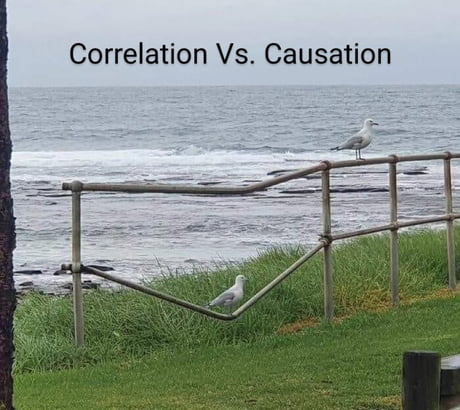
\includegraphics[width=\linewidth]{img/seagel.jpg}
        % \caption{Caption}
        % \label{fig:my_label}
    \end{figure}
    \end{column}
    \end{columns}
    
\end{itemize}

\end{viterbiframe}

\begin{viterbiframe}{{\alert{Spurious} correlations}}
    
    \begin{itemize}
        \item Determining if two sentences agree or contradict
        \item The presence of negation words like ‘\alert{never}’ is strongly correlated with contradiction 
        \item Artifacts in crowdsourced training data
    \end{itemize}
    
\end{viterbiframe}

\begin{viterbiframe}{{\alert{Spurious} correlations}}
    \begin{figure}
        \centering
        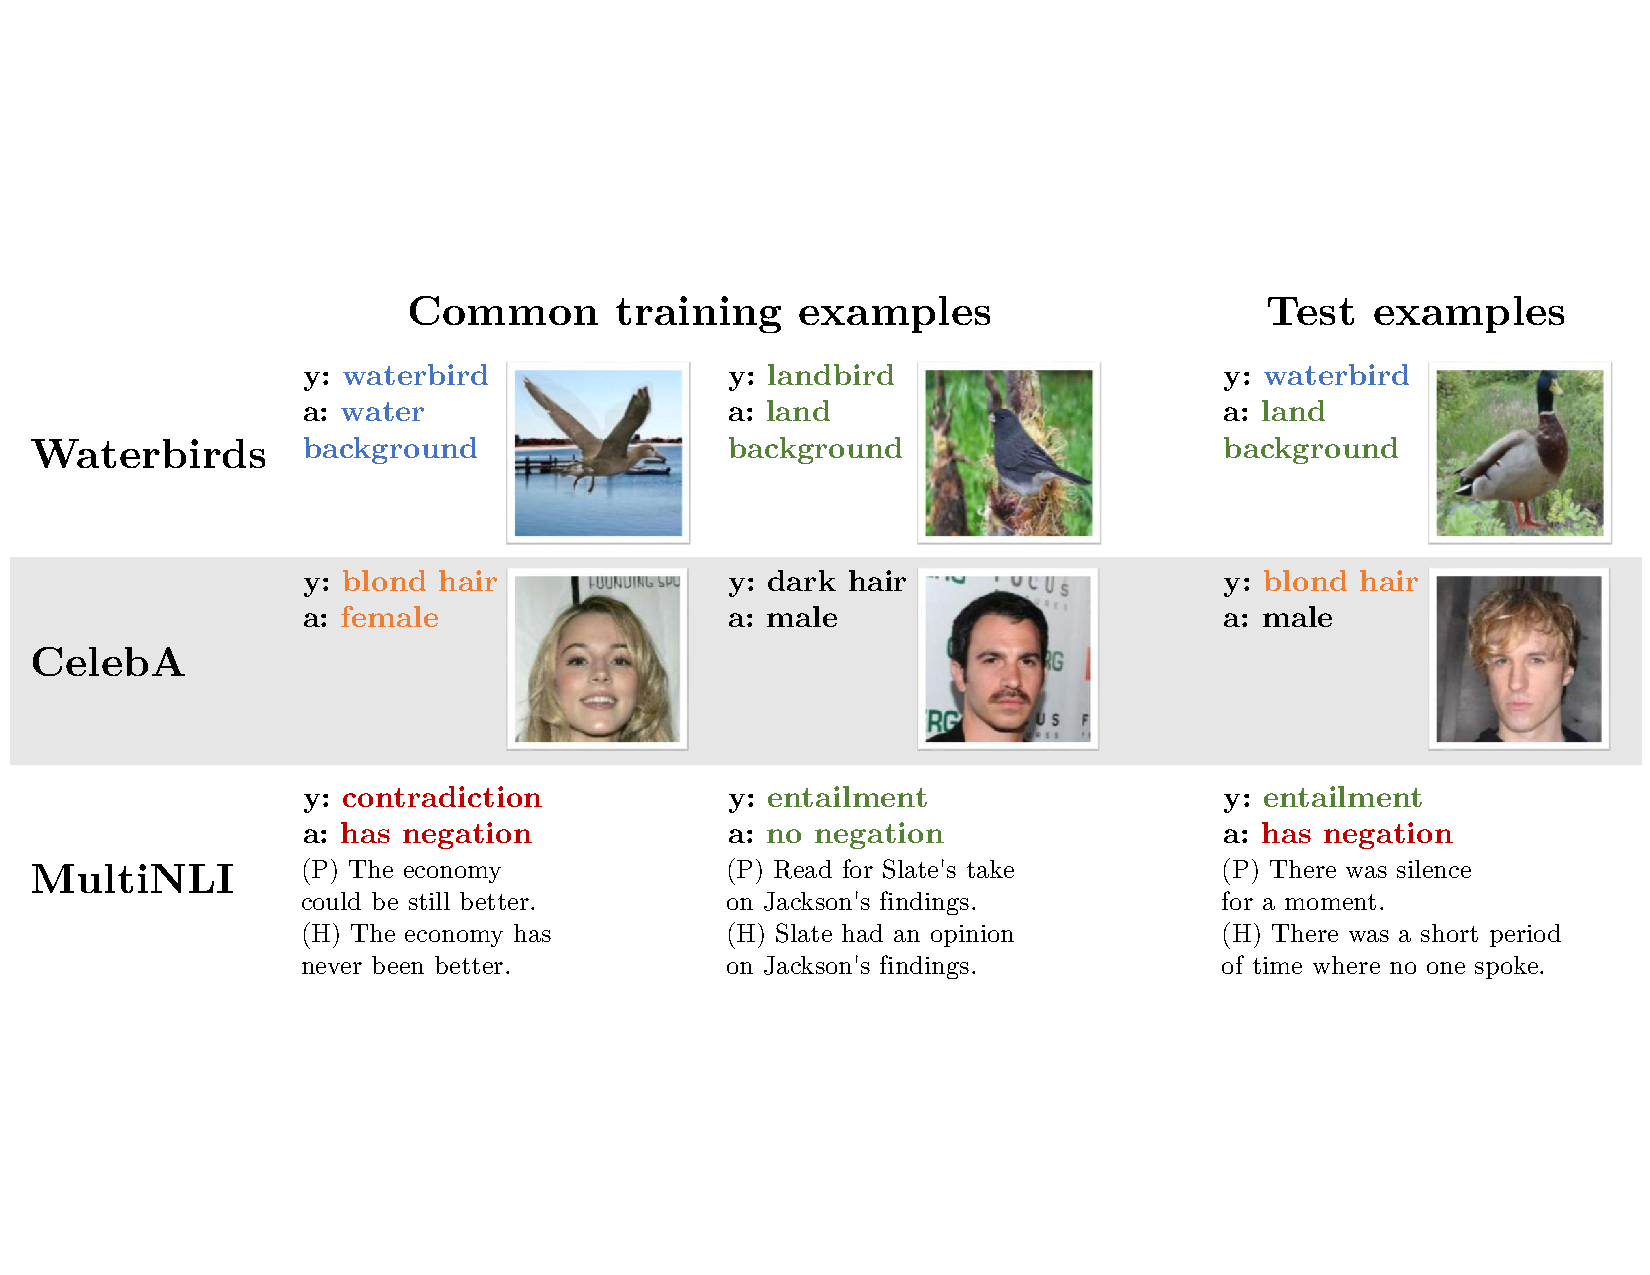
\includegraphics[width=\textwidth]{img/dataset.pdf}
        % \caption{}
        % \label{fig:my_label}
    \end{figure}
\end{viterbiframe}

\begin{viterbiframe}{Solution}
    \begin{itemize}
        \item Minimize the \alert{worst-case} loss over \alert{groups} in the training data
        \item i.e., Distributionally Robust Optimization \footcite{bental2013robust,oren2019distributionally}
        \item Grouping together \alert{contradictory} sentences with \alert{no negation} words in the \emph{natural language inference} (NLI) example above.
        
    \end{itemize}
\end{viterbiframe}

\begin{viterbiframe}{{Preliminary Experiments, DRO doesn't work}}
\begin{itemize}
    \item DRO in the context of \alert{overparameterized} neural networks in 3 applications
    \begin{itemize}
        \item NLI with the MultiNLI dataset %\footcite{williams2018broad}
        \item Facial recognition with CelebA %\footcite{liu2015deep}
        \item Bird photograph recognition with CUB dataset %\footcite{wah2011cub}.
    \end{itemize}
    \item Problem: if a model achieves \alert{zero training loss}, then it is optimal on both the worst-case (DRO) and the average training objectives:
    \begin{itemize}
        \item For both ERM and group DRO, the \alert{generalization gap} is small on average but large for the worst group.
    \end{itemize}
\end{itemize}
     
\end{viterbiframe}

\begin{viterbiframe}{Solution}

\begin{itemize}
    \item Use \alert{strongly-regularized} group DRO
    \pause
    \item Bi-product: Regularization might not be important for good \alert{average performance} e.g., models can \alert{“train longer and generalize better”} on average \footcite{hoffer2017train} 
    \pause
    \item It appears important for good worst-case performance.
\end{itemize}
\end{viterbiframe}

\section{Problem Setup}

\begin{viterbiframe}{{Objective Function}}
\begin{itemize}
    \item Empirical risk minimization (ERM):
    \begin{align}%\label{eqn:hterm}
      \hterm := \arg\min_{\theta \in \Theta} 
      \ \E_{(x, y) \sim \hP}
    [\ell(\theta; (x, y))]
    \end{align}
    where $\hP$ is the \alert{empirical distribution} over the training data.
    \end{itemize}
\end{viterbiframe}

\begin{viterbiframe}{{Objective Function}}
\begin{itemize}
    \item Distributionally Robust Optimization (DRO):
        \begin{align}\label{eq:dro}
          \underset{\theta \in \Theta}{\vphantom{\sup}\min} \Bigl\{ \mathcal{R}(\theta) := \sup_{Q \in \mathcal{Q}} \E_{(x, y) \sim Q}[\ell(\theta; (x, y))] \Bigr\}.
        \end{align}
        \pause
    The uncertainty set $\mathcal{Q}$ encodes the \alert{possible test distributions} that we want our model to perform well on.
    \end{itemize}
    \begin{figure}
        \centering
        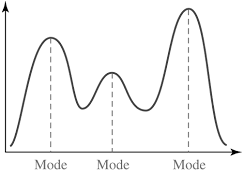
\includegraphics[width=.4\linewidth]{img/mmodal.png}
        % \caption{Caption}
        % \label{fig:my_label}
    \end{figure}
\end{viterbiframe}

\begin{viterbiframe}{Uncertainty Set}

\begin{itemize}
 \item Use \alert{Prior knowledge} of spurious correlations to \alert{define groups} over the training data
 
 \pause
 \item \alert{Group DRO}: the training distribution $P$ is assumed to be a mixture of $m$ groups $P_g$ indexed by $\mathcal{G} = \{1, 2, \ldots, m\}$.
 \pause
 \item Then 
 \[
 \mathcal{Q} := \{ \sum_{g=1}^m q_g P_g: q \in \Delta_m \}
 \]
 \pause
 \item and the worst-case risk is
 \begin{align}
\label{eqn:groupdroq}
  \mathcal{R}(\theta)
  &= \underset{g \in \mathcal{G}}{\max} \ \E_{(x, y) \sim P_g}[\ell(\theta; (x, y))].
\end{align} 
    by concavity of linear function.

\pause
 \item Learns models that are robust to \alert{group shifts}

\end{itemize}
 
\end{viterbiframe}  

\begin{viterbiframe}{Group DRO}
\begin{itemize}
    \item Assume the training data comprises $(x, y, g)$ triplets
    \pause
    \item Though we \alert{don't observe} $g$ at test time, so the model cannot use $g$ directly. 
    \pause
    \item Instead, worst-group risk $\hat{\mathcal{R}}(\theta)$:
    \begin{align}
    % \label{eqn:htdro}
      \htdro := \underset{\theta \in \Theta}{\vphantom{\sup}\argmin} \Bigl\{\hat{\mathcal{R}}(\theta) :=  \underset{g \in \mathcal{G}}{\vphantom{\argmin}\max} \ \E_{(x, y) \sim \hP_g}[\ell(\theta; (x, y))] \Bigr\}\nonumber
    \end{align}
    
    \item Worst-group \emph{generalization gap}
    \[\delta \eqdef  \mathcal{R}(\theta)  -\hat{\mathcal{R}}(\theta)\;,\]
    which for overparameterized neural networks, is large unless we apply \alert{sufficient regularization}.
\end{itemize}
\end{viterbiframe}


\begin{viterbiframe}{Application}
    Each data point $(x, y)$ has some \alert{input attribute} $a(x) \in \mathcal{A}$ that is spuriously correlated with the label $y$
    \pause
    
    We use this prior knowledge to \alert{form $m = |\mathcal{A}| \times |\mathcal{Y}|$} groups, one for each value of $(a, y)$.
    
    \pause
    
    
\end{viterbiframe}

\begin{viterbiframe}{Application}

\begin{itemize}

    \item Object recognition with correlated \alert{backgrounds}: Waterbirds
    
    $\mathcal{Y} = \{\text{waterbird}, \text{landbird}\}$
    
    $\mathcal{A} = \{\text{water background}, \text{land background}\}$,
    
    Waterbirds (landbirds) more frequently appearing against a water (land)
    
    \pause
    \item Object recognition with correlated \alert{demographics}: CelebA dataset
    
    $\mathcal{Y} = \{\text{blond}, \text{dark}\}$
    
    $\mathcal{A} = \{\text{male}, \text{female}\}$
    
    Smallest group: blond-haired males.
\end{itemize}
\end{viterbiframe}

\begin{viterbiframe}{Application (Cont.)}
\begin{itemize}
    \item NLI: MultiNLI dataset:
    
    Given \alert{hypothesis} is entailed by, neutral with, or contradicts a given \alert{premise}
    
    $\mathcal{Y} = \{\text{entailed}, \text{neutral}, \text{contradictory}\}$
    
    $\mathcal{A} = \{\text{no negation}, \text{negation}\}$
    
    Smallest group: entailment with negations
\end{itemize}
\end{viterbiframe}

\section{ERM vs. DRO}

\begin{viterbiframe}{ERM vs. group DRO}
\begin{itemize}
    \item Fine-tune ResNet50 models on Waterbirds and CelebA

\item Fine-tune BERT model on MultiNLI

\item SGD to train ERM

\item Special SGD to train group DRO

\end{itemize}


\end{viterbiframe}

\subsection{Both Have Poor Worst-group Acc}

\begin{viterbiframe}{Both Have Poor Worst-group Acc}

\begin{table}[]
    \centering
    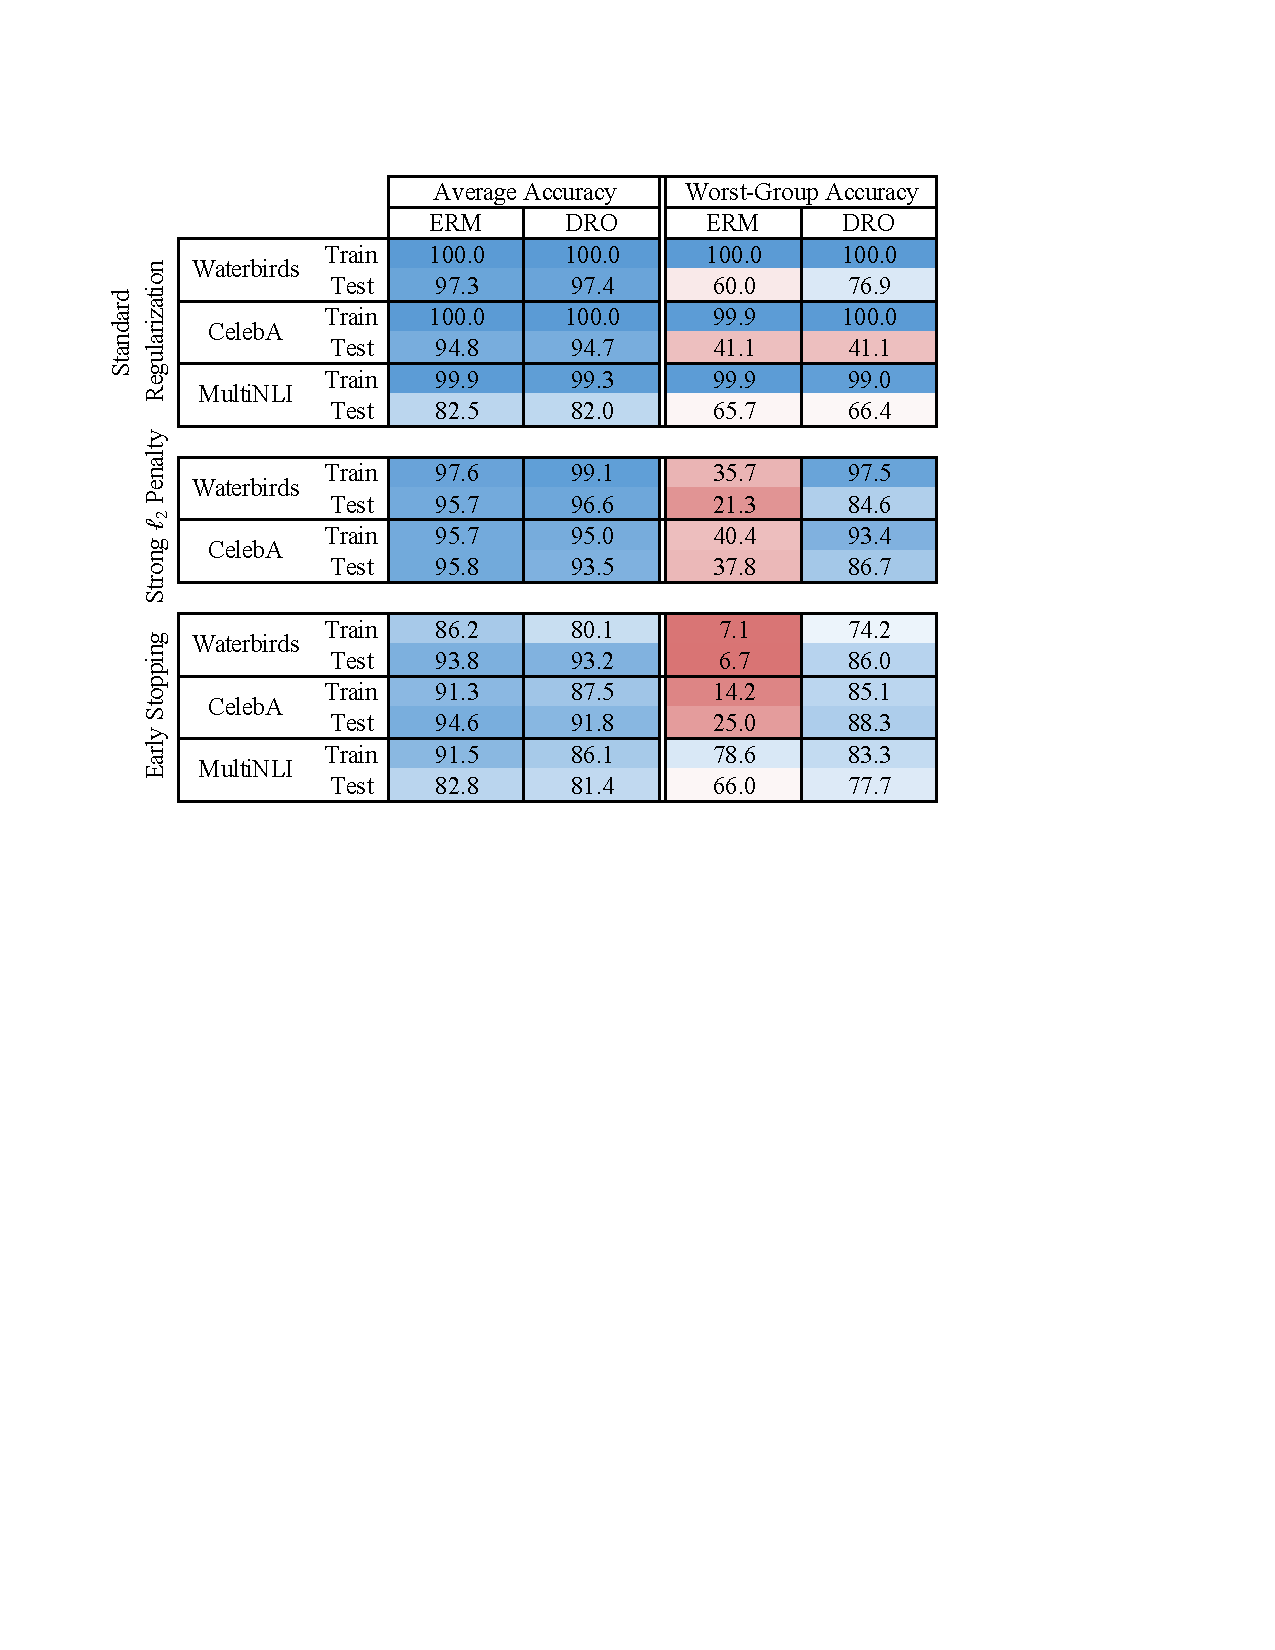
\includegraphics[width=.7\textwidth]{img/table_1.pdf}
    \caption{Cells are colored by accuracy, from low (red) to medium (white) to high (blue) accuracy}
    \label{tab:analysis}
\end{table}


\end{viterbiframe}

\begin{viterbiframe}{Both Have Poor Worst-group Acc}

\begin{figure}
    \centering
    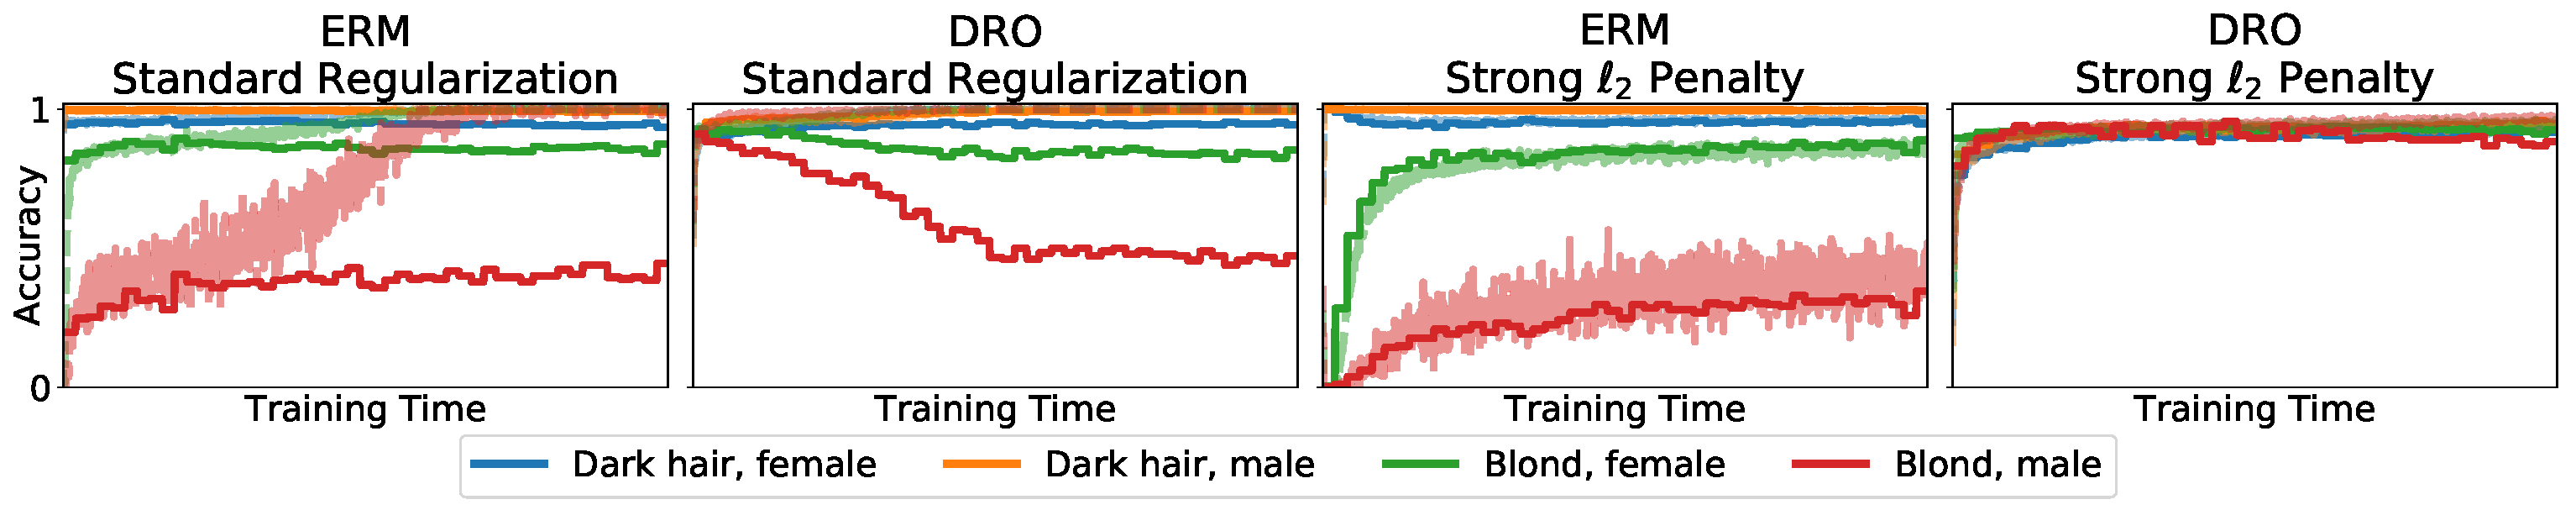
\includegraphics[width=\textwidth]{img/train_curve.pdf}
    \caption{Training (light) and validation (dark) accuracy for CelebA throughout training}
    % \label{fig:my_label}
\end{figure}

% If train using \alert{standard regularization} and hyperparameter settings

\begin{itemize}
    \item ERM and DRO have \alert{poor worst-group} accuracy in the overparameterized regime
    
    \item DRO \alert{improves worst-group} accuracy under appropriate regularization
\end{itemize}
\end{viterbiframe}

\subsection{DRO improves with Appropriate Regularization}
\begin{viterbiframe}{DRO improves with Appropriate Regularization}
    \begin{itemize}
        \item[1)] {\bf $\ell_2$ penalty}: Substantially reduces the \alert{generalization gap} for each group.
        
        Both still achieve high average test accuracies
        
        ERM poor worst-group Acc
        
        DRO improve worst-group Acc
        
        see Table~\ref{tab:analysis}
        
        \pause
        \item[2)] {\bf Early stopping}: Train each model for a \alert{fixed (small) number of epochs}
        
        Same as $\ell_2$
        
        Small \alert{drop} for DRO in Average test Acc
        
        see Table~\ref{tab:analysis}
    \end{itemize}
\end{viterbiframe}

\subsection{Group Adjustments Improves DRO}

\begin{viterbiframe}{Group Adjustments Improves DRO}
    
    \begin{itemize}
    \item
        Even with regularization, the \alert{generalization gap} vary across groups: 
        
        e.g., \alert{Train-test accuracy gap}, Waterbirds, DRO + strong $\Ltwo$ penalty: 
        
        Smallest group: $15.4\%$ 
        
        Largest group: $1.0\%$
        
        \pause
        \item So, at training time, \alert{prioritize} the groups that we \alert{expect to have a larger generalization gap}
        
        $\rightarrow$  Structural Risk Minimization \footcite{vapnik1992principles}.
    
    \end{itemize}
\end{viterbiframe}

\begin{viterbiframe}{Group-adjusted DRO Estimator}
    
    Generalization Gap \[\gengap = \E_{(x,y) \sim P_g}[\ell(\theta; (x,y))] - \E_{(x,y) \sim \hP_g}[\ell(\theta; (x,y))].\]
    
    use $\hatgengap=\frac{C}{\mathcal{Q}rt{n_g}}$, then \emph{Group-adjusted} DRO Estimator is
    \begin{align}\label{eqn:htadj}
        \htadj \eqdef \argmin_{\theta \in \Theta} \ \underset{g \in \mathcal{G}}{\vphantom{\argmin}\max} \ \left\{ \E_{(x, y) \sim \hP_g}[\ell(\theta; (x, y))] + \frac{C}{\mathcal{Q}rt{n_g}}\right\}.
    \end{align}
\end{viterbiframe}

\begin{viterbiframe}{Group-adjusting Improves DRO}
    
    \begin{table}
    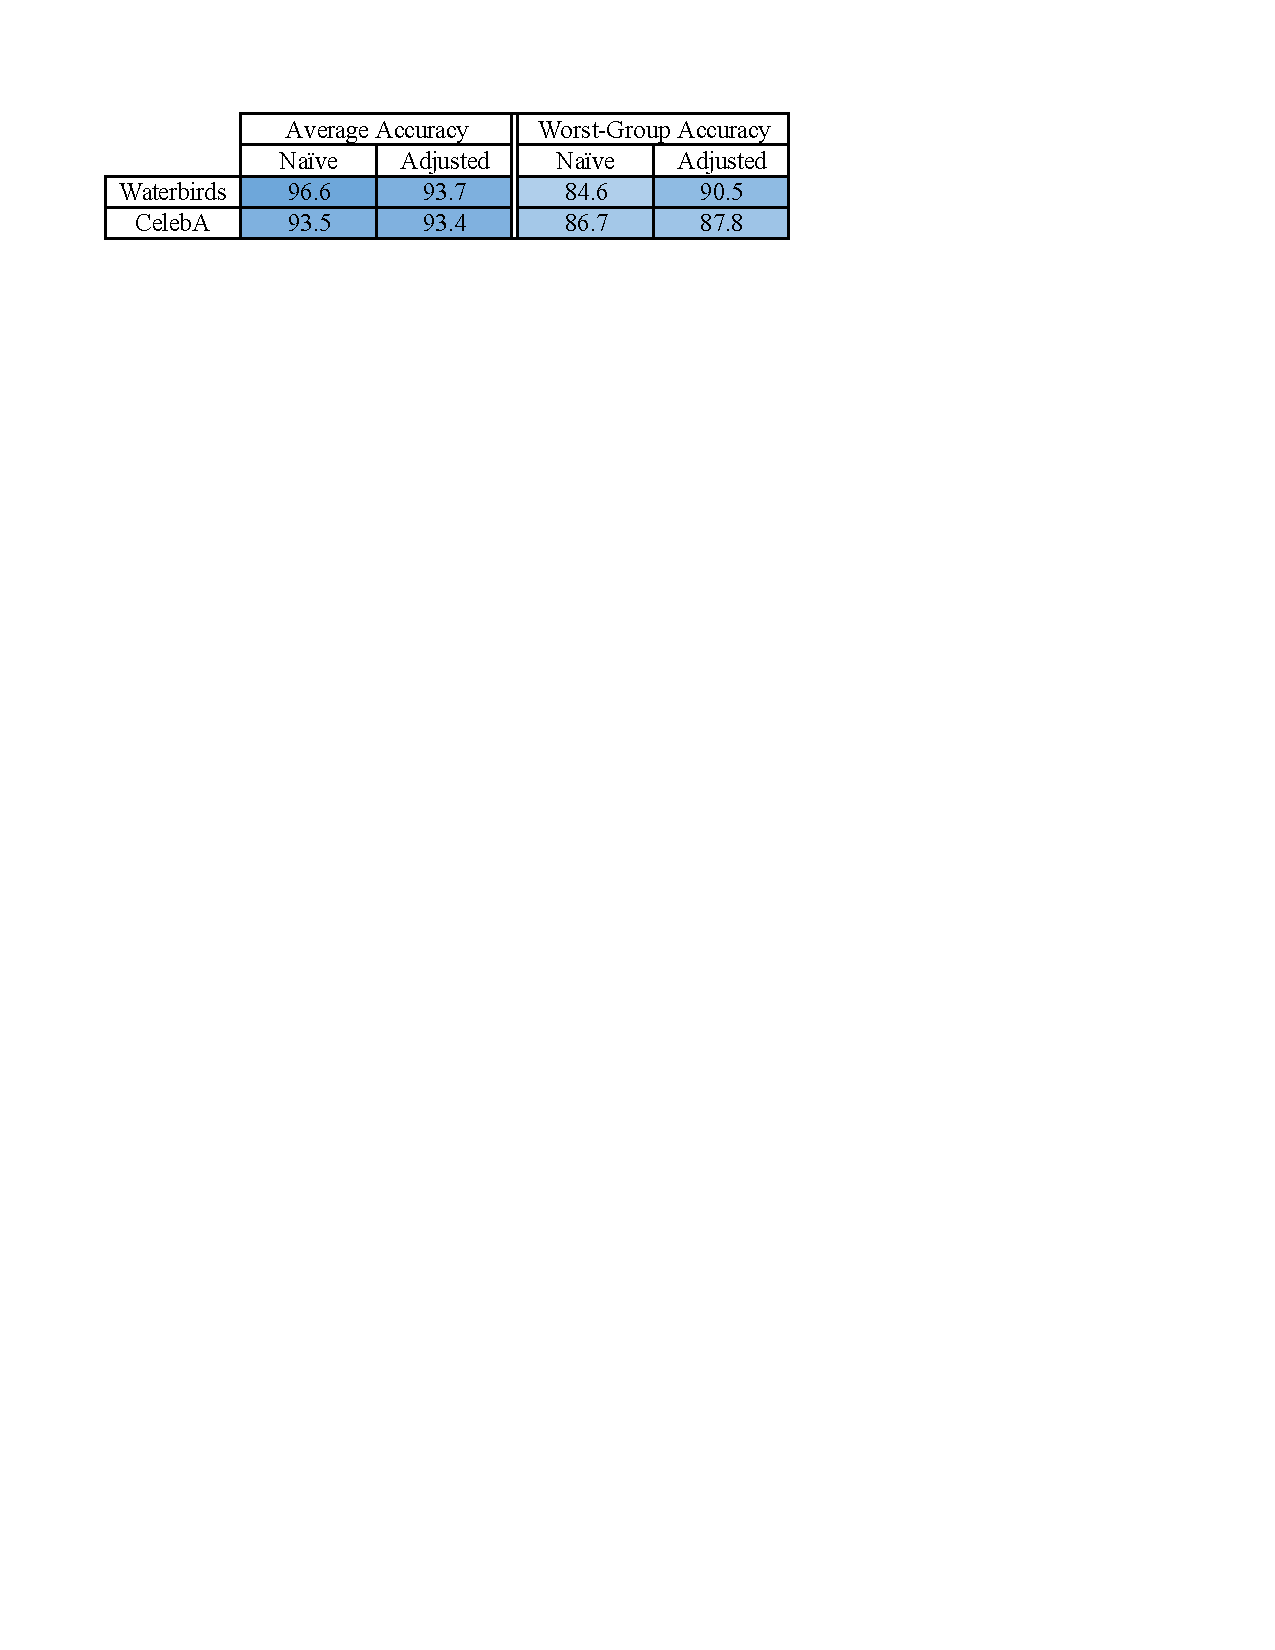
\includegraphics[width=0.8\textwidth]{img/table_2.pdf}
    % \caption{Average and worst-group test accuracies with and without group adjustments. Group adjustments improve worst-group accuracy, though average accuracy drops for Waterbirds.}
    % \label{tab:adj}
    \end{table}

    \begin{figure}
      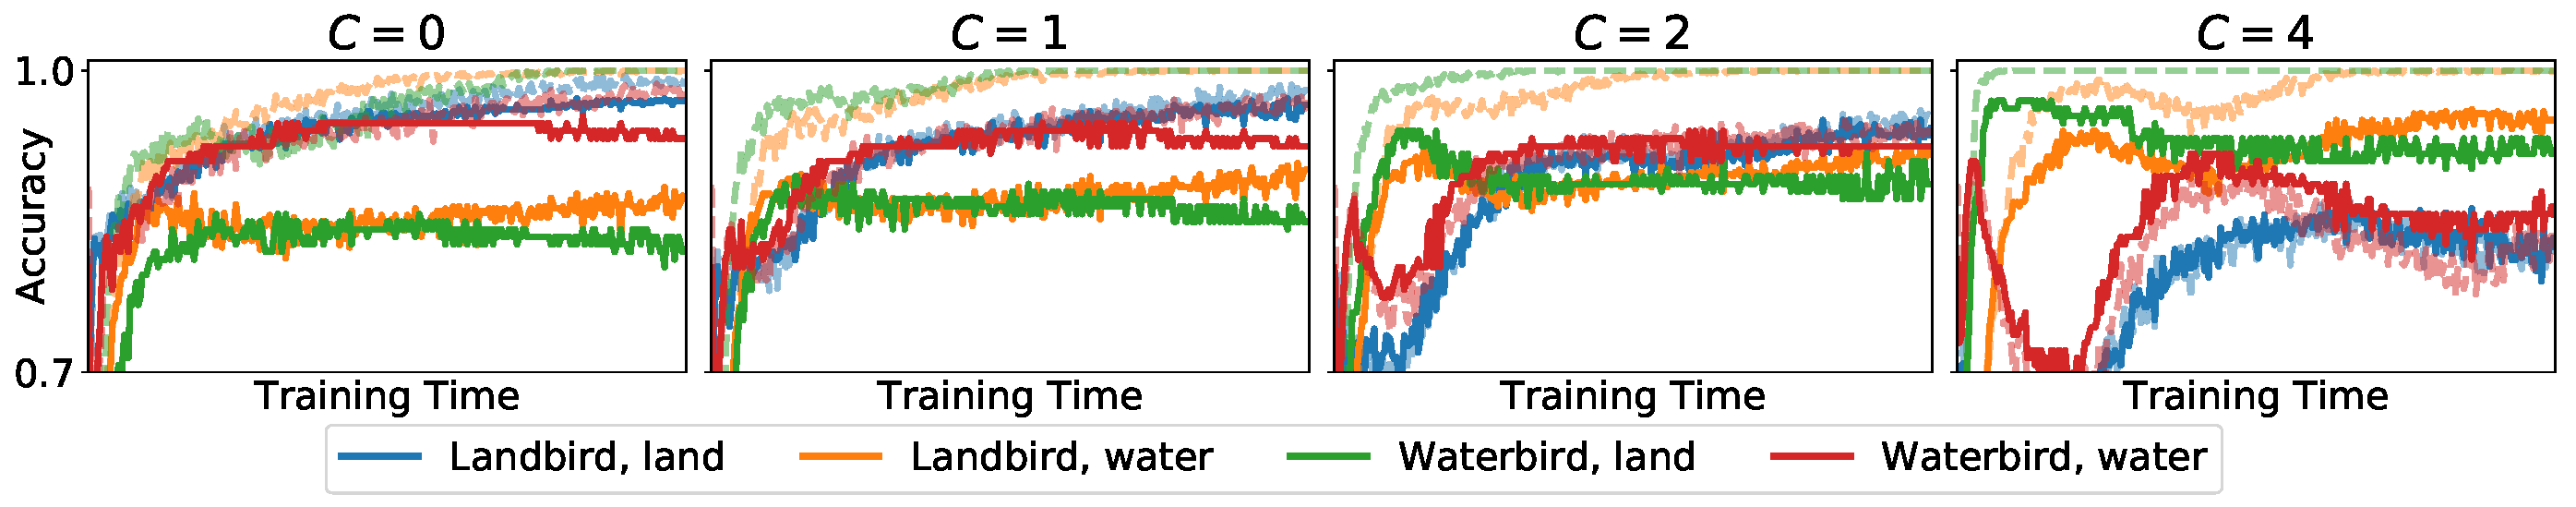
\includegraphics[width=\textwidth]{img/group_adj_waterbirds.pdf}
      \caption{
        Training (light) and validation (dark) accuracies for each group over time,
        for different adjustments $C$.
        % When $C=0$, the generalization gap for waterbirds on land (green line) is large, dragging down worst-group accuracy.
        At $C=2$, which has the best worst-group validation accuracy, the accuracies are balanced.
        % At $C=4$, we overcompensate for group sizes, so smaller groups (e.g., waterbirds on land) do better at the expense of larger groups (e.g., landbirds on land).
    }
    \label{fig:adj}
    \end{figure}

\end{viterbiframe}

\section{DRO vs. IW}

\begin{viterbiframe}{DRO vs. Importance Weighting}
    Importance-weighted estimator learn
    \begin{align}
      \htw \eqdef \argmin_{\theta \in \Theta} \ \E_{(x,y,g) \sim \hP}[w_g \ \ell(\theta; (x, y))].
    \end{align}
    for $w \in \Delta_m$.

    \pause
    Take $w_g = 1 / \E_{g^\prime \sim \hP} [\1(g^\prime = g)]$.
\end{viterbiframe}
    
\subsection{Empirical Comparison}
\begin{viterbiframe}{Empirical Comparison}
        \begin{table}[th]
        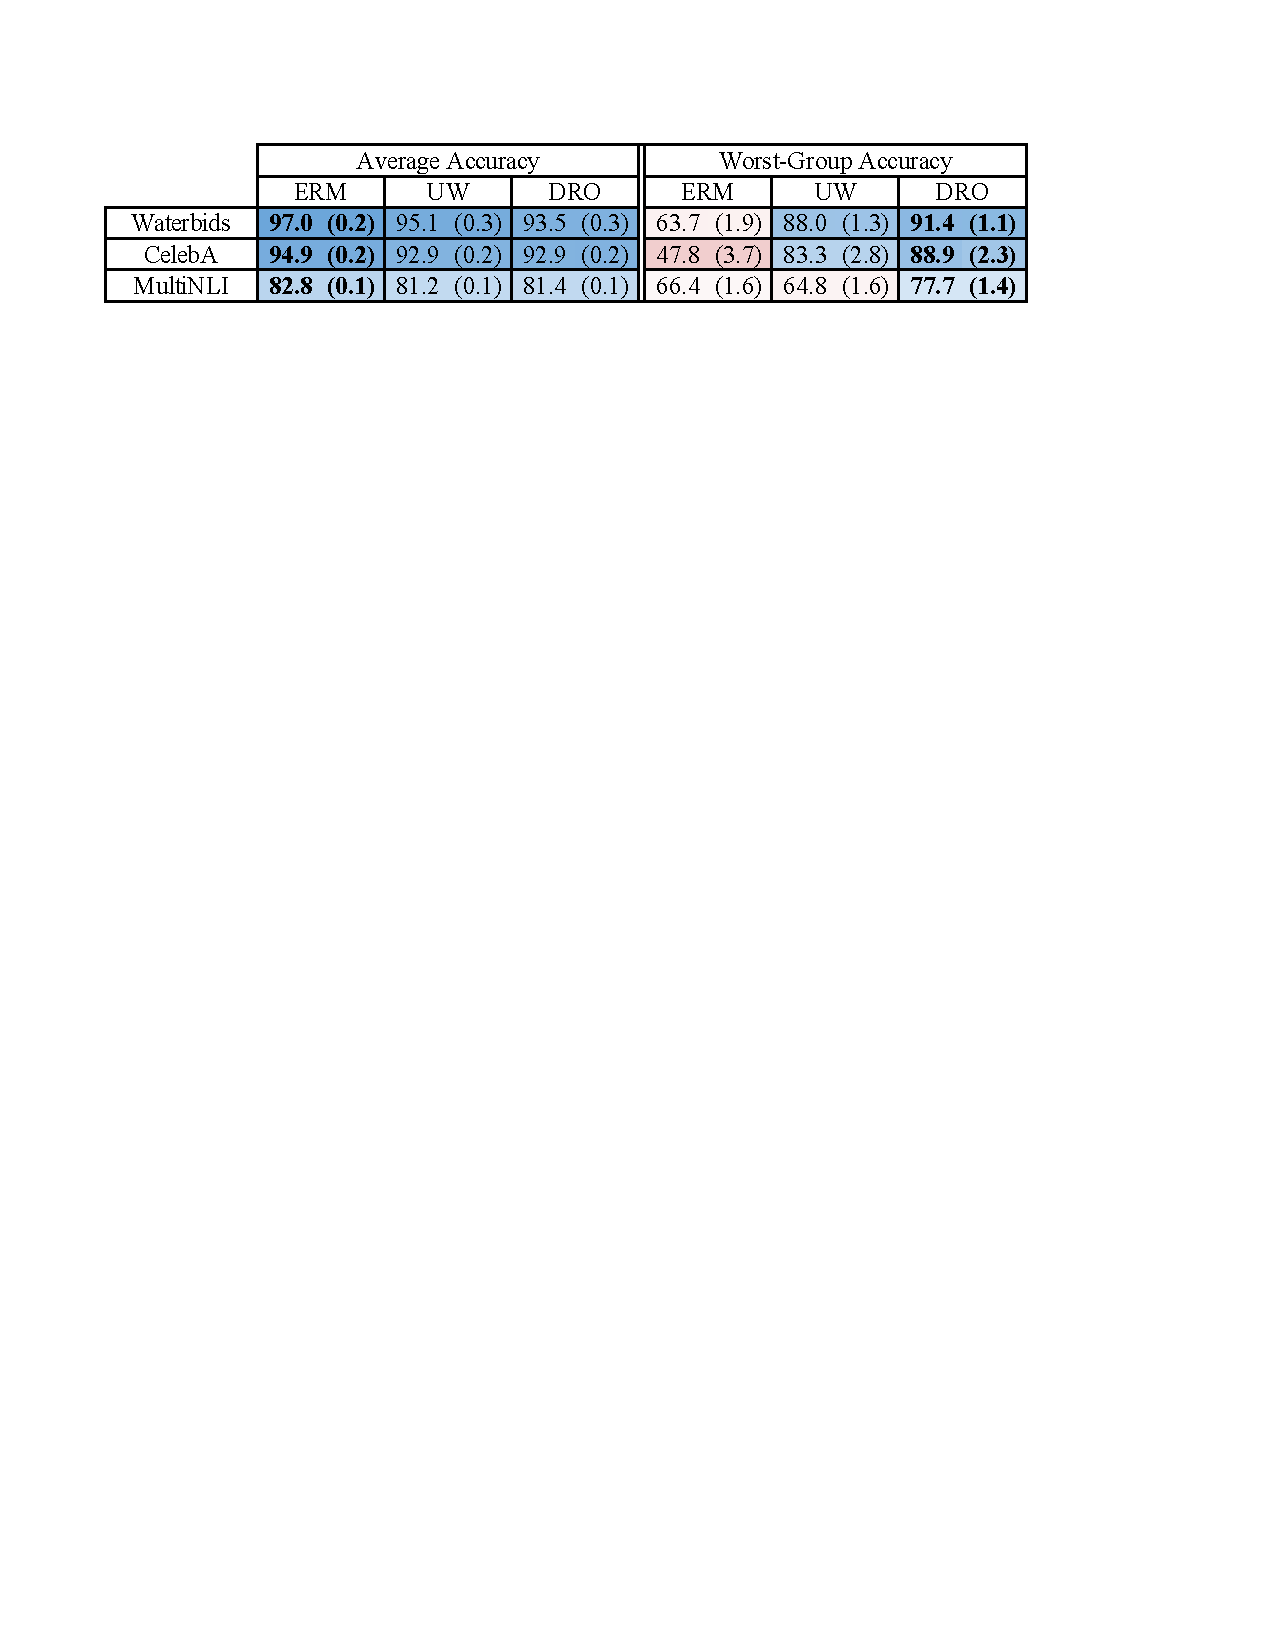
\includegraphics[width=\textwidth]{img/table_3.pdf}
        \caption{Comparison of ERM, upweighting (UW), and group DRO models.
        % , with binomial standard deviation in parenthesis. For each objective, we grid search over $\Ltwo$ penalty strength, number of epochs, and group adjustments and report on the model with highest validation accuracy.
        % These numbers differ from the previous tables because of the larger grid search.
          }
        \label{tab:benchmark}
        \end{table}
\end{viterbiframe}

\subsection{Theoretical comparison}
\begin{viterbiframe}{Theoretical comparison}

    \begin{itemize}
        \item IW and DRO can learn equivalent models in the \alert{convex} setting under some importance weights 
        
        \pause
        % \item 
        \begin{proposition}\label{prop:convex-reweight}
          Suppose that the loss $\ell(\cdot; z)$ is \alert{continuous} and \alert{convex} for all $z$ in $\mathcal{Z}$,
          and let the uncertainty set $\mathcal{Q}$ be a set of distributions supported on $\mathcal{Z}$.
          Assume that $\mathcal{Q}$ and the model family $\Theta \subseteq \R^d$ are \alert{convex} and \alert{compact},
          and let $\theta^* \in \Theta$ be a \alert{minimizer of the worst-group} objective $\mathcal{R}(\theta)$.
          Then there exists a distribution $Q^* \in \mathcal{Q}$ such that $\theta^* \in \argmin_\theta \E_{z \sim Q^*} [\ell(\theta;z)]$.
        \end{proposition}
        \begin{proof}
        Linear program duality.
        \end{proof}
        
        \item Not necessarily when the models are \alert{non-convex}.
    \end{itemize}
\end{viterbiframe}

\begin{viterbiframe}{Non-convex Case}
Counter Example
\begin{figure}[th]
      \centering
      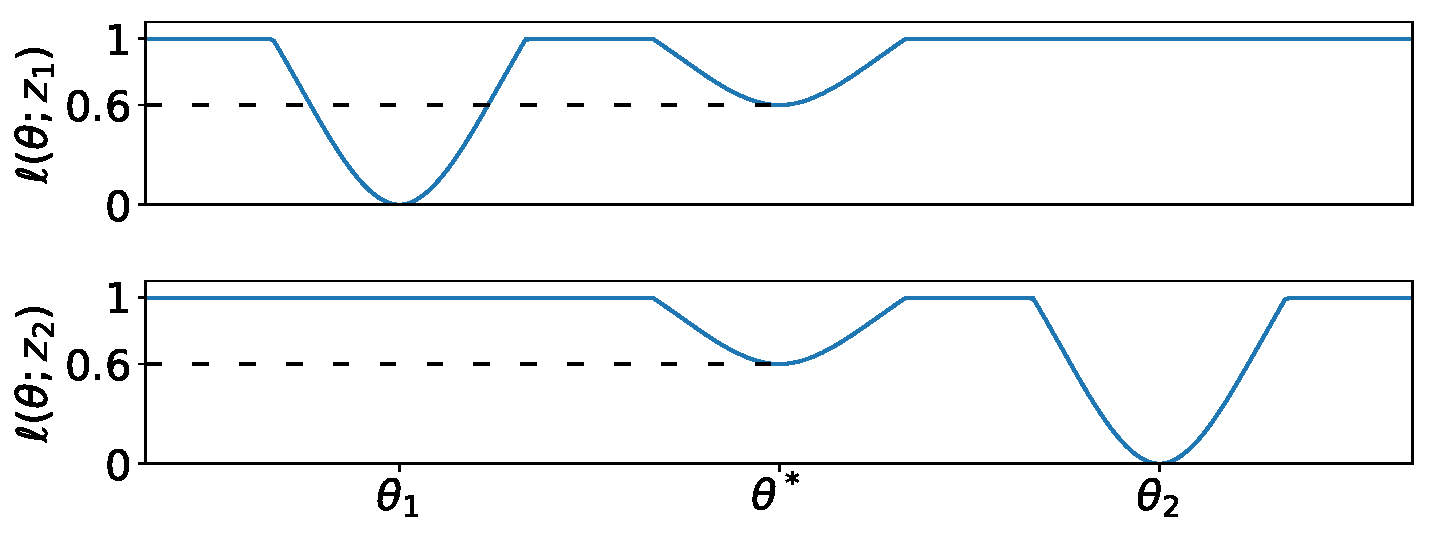
\includegraphics[width=0.8\textwidth]{img/counterexample.pdf}
      \caption{
        Toy example illustrating that \alert{DRO} and \alert{importance weighting} are \alert{not equivalent}. The DRO solution is $\theta^*$, while any importance weighting would result in solutions at $\theta_1$ or $\theta_2$.
      }\label{fig:DRO_counterexample}
    \end{figure}
\end{viterbiframe}

\section{Algorithm}
\begin{viterbiframe}{Training DRO}
    Prvious work: two \alert{stochastic} optimization methods for \alert{general non-convex} DRO:
    \begin{itemize}
        \item[(i)] Stochastic gradient descent (SGD) on the \alert{Lagrangian dual} of the objective: fails for group DRO 
        \item[(ii)] Direct \alert{minimax} optimization 
    \end{itemize}
    
    Rewrite the DRO as
    \begin{align}
      \min_{\theta \in \Theta} \sup_{q \in \Delta_m} \ \sum_{g=1}^m q_g \E_{(x, y) \sim P_g}[\ell(\theta; (x, y))].
    \end{align}
\end{viterbiframe}

\begin{viterbiframe}{Algorithm}
    \small{
    \begin{algorithm}[H]
    \label{alg:opt}
     \DontPrintSemicolon
     \KwIn{Step sizes $\eta_q, \eta_\theta; P_g$ for each $g\in \gset$}
     Initialize $\theta\iter{0}$ and $\padv\iter{0}$\;
     \For{$t=1,\dots,T$}{
      $ g \sim \text{Uniform}(1,\dots,\ngroup)$ \tcp*{Choose a group $g$ at random}
      $ x,y \sim P_g$ \tcp*{Sample $x, y$ from group $g$}
      $ \padv^\prime \gets \padv\iter{t-1}$;\
      $ \padv^\prime_g \gets \padv^\prime_g\exp({\eta_q\ell(\theta\iter{t-1}; (x,y))})$ \tcp*{Update weights for group $g$}
      $ \padv\iter{t} \gets \padv^\prime / \sum_{g^\prime} \padv^\prime_{g^\prime}$ \tcp*{Renormalize $q$}
      $\theta\iter{t} \gets \theta\iter{t-1} - \eta_\theta \padv_g^{(t)}\nabla \ell(\theta\iter{t-1}; (x,y))$ \tcp*{Use $q$ to update $\theta$}
     }
      \caption{Online optimization algorithm for group DRO}
    \end{algorithm}
    }
    Has a convergence rate $1/\sqrt{T}$ in the convex setting.
\end{viterbiframe}


\section{Conclusion}
\begin{viterbiframe}{Discussion}
    \begin{itemize}
        \item What to do when groups are imperfectly specified? e.g., No prior knowledge, or training groups are ill defined for the test time.
        
        \item Regarding Average vs. Worst-case generalization in NNs, what other tools can you think of to analyze/address the trade-off?
    \end{itemize}
\end{viterbiframe}

\section{Fair w/o Demogs}
\begin{viterbiframe}{{Paper Intro}}
\begin{itemize}
    \item {\bf Fairness Without Demographics in Repeated Loss Minimization}
    \begin{itemize}
        {\small
        \item[] Tatsunori B. Hashimoto, \textit{\scriptsize Stanford University}
        \item[] Megha Srivastava, \textit{\scriptsize Stanford University}
        \item[] Hongseok Namkoong, \textit{\scriptsize Stanford University}
        \item[] Percy Liang, \textit{\scriptsize Stanford University}}
    \end{itemize}
\end{itemize}
% We follow the current of the paper.
\end{viterbiframe}

\begin{viterbiframe}{Introduction}
    \begin{itemize}
        \item Minimize average loss $~\rightarrow~$ Representation disparity
        \pause
        \item Acc effects \emph{use retention}: a minority group can shrink over time.
        \pause
        \item ERM amplifies representation disparity
        \pause
        \item Minimizes the \emph{worst case risk} 
        \pause
        over all distributions close to the empirical distribution.
        \item This controls the risk of the minority group, while remaining oblivious to the identity of the groups
        
    \end{itemize}
    
\end{viterbiframe}

\end{document}
